% interactcadsample.tex
% v1.04 - May 2023

\documentclass[]{interact}

\usepackage{epstopdf}% To incorporate .eps illustrations using PDFLaTeX, etc.
\usepackage{subfigure}% Support for small, `sub' figures and tables
%\usepackage[nolists,tablesfirst]{endfloat}% To `separate' figures and tables from text if required

\usepackage{natbib}% Citation support using natbib.sty
\bibpunct[, ]{(}{)}{;}{a}{}{,}% Citation support using natbib.sty
\renewcommand\bibfont{\fontsize{10}{12}\selectfont}% Bibliography support using natbib.sty

\theoremstyle{plain}% Theorem-like structures provided by amsthm.sty
\newtheorem{theorem}{Theorem}[section]
\newtheorem{lemma}[theorem]{Lemma}
\newtheorem{corollary}[theorem]{Corollary}
\newtheorem{proposition}[theorem]{Proposition}

\theoremstyle{definition}
\newtheorem{definition}[theorem]{Definition}
\newtheorem{example}[theorem]{Example}

\theoremstyle{remark}
\newtheorem{remark}{Remark}
\newtheorem{notation}{Notation}


% tightlist command for lists without linebreak
\providecommand{\tightlist}{%
  \setlength{\itemsep}{0pt}\setlength{\parskip}{0pt}}



\usepackage{lscape}
\usepackage{hyperref}
\usepackage[utf8]{inputenc}
\def\tightlist{}
\usepackage{setspace}
\doublespacing

\usepackage{booktabs}
\usepackage{longtable}
\usepackage{array}
\usepackage{multirow}
\usepackage{wrapfig}
\usepackage{float}
\usepackage{colortbl}
\usepackage{pdflscape}
\usepackage{tabu}
\usepackage{threeparttable}
\usepackage{threeparttablex}
\usepackage[normalem]{ulem}
\usepackage{makecell}
\usepackage{xcolor}

\begin{document}


\articletype{}

\title{Automated Assessment of Residual Plots with Computer Vision
Models}


\author{\name{Weihao Li$^{a, b}$, Dianne Cook$^{a}$, Emi Tanaka$^{a, b,
c}$, Susan VanderPlas$^{d}$, Klaus Ackermann$^{a}$}
\affil{$^{a}$Department of Econometrics and Business Statistics, Monash
University, Clayton, VIC, Australia; $^{b}$Biological Data Science
Institute, Australian National University, Acton, ACT,
Australia; $^{c}$Research School of Finance, Actuarial Studies and
Statistics, Australian National University, Acton, ACT,
Australia; $^{d}$Department of Statistics, University of Nebraska,
Lincoln, Nebraska, USA}
}


\maketitle

\begin{abstract}
Plotting the residuals is a recommended procedure to diagnose deviations
from linear model assumptions, such as non-linearity,
heteroscedasticity, and non-normality. The presence of structure in
residual plots can be tested using the lineup protocol to do visual
inference. There are a variety of conventional residual tests, but the
lineup protocol, used as a statistical test, performs better for
diagnostic purposes because it is less sensitive and applies more
broadly to different types of departures. However, the lineup protocol
relies on human judgment which limits its scalability. This work
presents a solution by providing a computer vision model to automate the
assessment of residual plots. It is trained to predict a distance
measure that quantifies the disparity between the residual distribution
of a fitted classical normal linear regression model and the reference
distribution, based on Kullback-Leibler divergence. Evaluation using
data from a prior human-subject experiment shows the model exhibits
lower sensitivity than conventional tests but higher sensitivity than
human visual tests. Several examples from classical papers and
contemporary data demonstrate the method's paractical utility in
automating residual diagnostics.
\end{abstract}

\begin{keywords}
statistical graphics; data visualization; visual inference; computer
vision; machine learning; hypothesis testing; reression analysis;
cognitive perception; simulation; practical significance
\end{keywords}

\section{Introduction}\label{sec-model-introduction}

Plotting residuals is commonly regarded as a standard practice in linear
regression diagnostics \citep{belsley1980regression, cook1982residuals}.
This visual assessment plays a crucial role in identifying whether key
model assumptions, such as linearity, homoscedasticity, and normality,
are reasonable. It also helps in understanding the goodness of fit and
various unexpected characteristics of the model.

Generating a residual plot in most statistical software is often as
straightforward as executing a line of code or clicking a button.
However, accurately interpreting a residual plot can be challenging. A
residual plot can exhibit various visual features, but it is crucial to
recognize that some may arise from the characteristics of predictors and
the natural stochastic variation of the observational unit, rather than
indicating a violation of model assumptions \citep{li2024plot}. Consider
Figure \ref{fig:false-finding} as an example, the residual plot displays
a triangular left-pointing shape. The distinct difference in the spread
of the residuals across the fitted values may result in the analyst
suggesting that there may be heteroskedasticity, however, it is
important to avoid over-interpreting this visual pattern. In this case,
the fitted regression model is correctly specified, and the triangular
shape is actually a result of the skewed distribution of the predictors,
rather than indicating a flaw in the model.

The concept of visual inference, as proposed by
\citet{buja2009statistical}, provides an inferential framework to assess
whether residual plots indeed contain visual patterns inconsistent with
the model assumptions. The fundamental idea involves testing whether the
true residual plot visually differs significantly from null plots, where
null plots are plotted with residuals generated from the residual
rotation distribution \citep{langsrud2005rotation}, which is a
distribution consistent with the null hypothesis \(H_0\) that the linear
regression model is correctly specified. Typically, the visual test is
accomplished through the lineup protocol, where the true residual plot
is embedded within a lineup alongside several null plots. If the true
residual plot can be distinguished from the lineup, it provides evidence
for rejecting \(H_0\).

The practice of delivering a residual plot as a lineup is generally
regarded as a valuable approach. Beyond its application in residual
diagnostics, the lineup protocol has been integrated into the analysis
of diverse subjects. For instance, Loy and Hofmann
\citetext{\citeyear{loy2013diagnostic}; \citeyear{loy2014hlmdiag}; \citeyear{loy2015you}}
illustrated its applicability in diagnosing hierarchical linear models.
Additionally, \citet{widen2016graphical} and \citet{fieberg2024using}
demonstrated its utility in geographical and ecology research
respectively, while \citet{krishnan2021hierarchical} explored its
effectiveness in forensic examinations.

A practical limitation of the lineup protocol lies in its reliance on
human judgements \citep[see][ about the practical
limitations]{li2024plot}. Unlike conventional statistical tests that can
be performed computationally in statistical software, the lineup
protocol requires human evaluation of images. This characteristic makes
it less suitable for large-scale applications, given the associated high
labour costs and time requirements. There is a substantial need to
develop an approach to substitute these human judgement with an
automated reading of data plots using machines.

Efforts to automate plot interpretation date back to early work like
Tukey's ``Scagnostics'' \citep{tukey1985computer}, which is a set of
numerical statistics that summarize features of scatter plots.
\citet{wilkinson2005graph} expanded on this work, introducing
scagnostics based on computable measures applied to planar proximity
graphs. These measures, including, but not limited to, ``Outlying'',
``Skinny'', ``Stringy'', ``Straight'', ``Monotonic'', ``Skewed'',
``Clumpy'', and ``Striated'', aimed to characterize outliers, shape,
density, trend, coherence and other characteristics of the data.
However, as noted by \citet{buja2009statistical}, such measures may not
capture the full range of visual patterns necessary for residual
diagnostics. A more promising direction lies in enabling computers to
learn the relevant visual features directly mirroring how humans
intuitively interpret plots.

Modern computer vision models are well-suited for addressing this
challenge. They rely on deep neural networks with convolutional layers
\citep{fukushima1982neocognitron}. These layers use small, sliding
windows to scan the image, performing a dot product to extract local
features and patterns. Numerous studies have demonstrated the efficacy
of convolutional layers in addressing various vision tasks, including
image recognition \citep{rawat2017deep}. Despite the widespread use of
computer vision models in fields like computer-aided diagnosis
\citep{lee2015image}, pedestrian detection \citep{brunetti2018computer},
and facial recognition \citep{emami2012facial}, their application in
reading data plots remains limited. While some studies have explored the
use of computer vision models for tasks such as reading recurrence plots
for time series regression \citep{ojeda2020multivariate}, time series
classification
\citep{chu2019automatic, hailesilassie2019financial, hatami2018classification, zhang2020encoding},
anomaly detection \citep{chen2020convolutional}, and pairwise causality
analysis \citep{singh2017deep}, the application of reading residual
plots with computer vision models is a new field of study.

In this paper, we develop computer vision models and integrate them into
the residual plots diagnostics workflow, addressing the need for an
automated visual inference. The paper is structured as follows. Section
\ref{sec-model-specifications} discusses various specifications of the
computer vision models. Section
\ref{sec-model-distance-between-residual-plots} defines the distance
measure used to detect model violations, while Section
\ref{sec-model-distance-estimation} explains how the computer vision
models estimate this distance measure. Section
\ref{sec-model-statistical-testing} covers the statistical tests based
on the estimated distance. Sections \ref{sec-model-architecture} and
\ref{sec-model-data-generation} describe the model architecture and the
corresponding data generation and training process, respectively. The
results are presented in Section \ref{sec-model-results}. Example
dataset applications are discussed in Section \ref{sec-examples}.
Finally, we conclude with a discussion of our findings and propose ideas
for future research directions.

\begin{figure}[!h]

{\centering 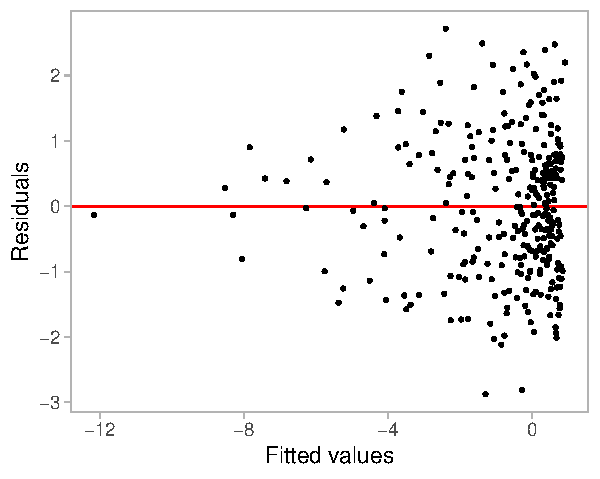
\includegraphics[width=0.5\linewidth]{paper_files/figure-latex/false-finding-1} 

}

\caption{An example residual vs fitted values plot (red line indicates 0 corresponds to the x-intercept, i.e. $y=0$). The vertical spread of the data points varies with the fitted values. This often indicates the existence of heteroskedasticity, however, here the result is due to skewed distribution of the predictors rather than heteroskedasticity. The Breusch-Pagan test rejects this residual plot at 95\% significance level ($p\text{-value} = 0.046$).}\label{fig:false-finding}
\end{figure}

\section{Model Specifications}\label{sec-model-specifications}

There are various specifications of the computer vision model that can
be used to assess residual plots. We discuss these specifications below
focusing on two key components of the model formula: the input and the
output format.

\subsection{Input Formats}\label{input-formats}

Deep learning models are sensitive to input design, and several
alternatives are available for encoding residual plots.

A simple approach involves feeding vectors of residuals and fitted
values into the model. While this format contains all relevant
information, the input length varies with sample size, which conflicts
with the fixed-shape requirements of modern vision models such as those
implemented in TensorFlow \citep{abadi2016tensorflow}. Padding can be
used to enforce uniform length but risks truncation if inputs exceed the
fixed size. Alternatively, fixed-size sampling of residual--fitted value
pairs can ensure consistency, though at the cost of some information
loss.

Another strategy is to convert residual plots into images. This enables
the use of standard convolutional architectures such as VGG16
\citep{simonyan2014very}, which can effectively capture spatial
patterns. Although discretization introduces some losses in detail,
image-based inputs offer a richer representation by preserving the joint
distribution of residuals and fitted values in a visually interpretable
format. To ensure model generalization, it is essential to use residual
plots in a consistent style, i.e., same aesthetics, layout, scaling and
color schemes.

Using multiple residual plots as input, such as pairs, triplets, or full
lineups is also a possible option. For instance, triplet networks
\citep{chopra2005learning} can assess visual similarity if we assume
null plots are more similar from each other than from the true residual
plot, which may help distinguish null plots from true residual plots.
However, these architectures introduce complexity in training due to
weight sharing and specialized loss functions. We experimented with this
setting in a pilot study, and found multiple residual plots led to high
input resolution, high computational cost and suboptimal model
performance.

Balancing accuracy, interpretability, and implementation cost, we adopt
a single residual plot in image format as the model input.

\subsection{Output Formats}\label{output-formats}

Given the input is a single fixed-resolution image, the model output can
be defined for various tasks, including binary classification,
multiclass classification, and numeric regression.

In the binary case, the outcome may indicate whether the input image is
consistent with a null plot, as determined either by (1) the
data-generating process or (2) the outcome of a visual test based on
human judgment. The first approach models the probability that a
residual plot is not a null plot and is a viable option. In contrast,
the second relies on experimental data that are often scarce or
inconsistent across studies.

Alternatively, a multiclass outcome may classify images into categories
such as ``contains outliers'' vs.~``does not contain outliers'' or ``is
non-linear'' vs.~``not non-linear,'' among other diagnostic features.
While this approach is appealing in theory, it essentially reverts to
the traditional testing framework, where tests focus on detecting
specific types of model violations in isolation.

A third option is to produce a meaninful and interpretable numerical
measure that quantifies the strength of suspicious visual patterns
reflecting the extent of model violations, or the difficulty index for
identifying whether a residual plot has no issues. However, such
measures are often used informally in daily communications but rarely
formalized. For supervised learning, they must be clearly defined and
reliably estimable.

In this study, we defined and used a continuous distance between a true
residual plot and a theoretically ``good'' residual plot. This approach
captures the degree to which a plot deviates from model assumptions. In
contrast, a probability output based on binary labels, where true
residual plots are labeled as 1 and null plots as 0, cannot express the
severity of violation. It forces the model to infer this information
solely from the data distribution, which may be inefficient and discards
useful prior knowledge.

\section{Distance from a Theoretically ``Good'' Residual
Plot}\label{sec-model-distance-between-residual-plots}

To develop a computer vision model for assessing residual plots within
the visual inference framework, it is important to precisely define a
numerical measure of ``difference'' or ``distance'' between plots. This
distance can take the form of a basic statistical operation on pixels,
such as the sum of square differences, however, a pixel-to-pixel
comparison makes little sense in comparing residual plots where the main
interest would be structural patterns. Alternatively, it could involve
established image similarity metrics like the Structural Similarity
Index Measure \citep{wang2004image} which compares images by integrating
three perception features of an image: contrast, luminance, and
structure (related to average, standard deviation and correlation of
pixel values over a window, respectively). These image similarity
metrics are tailored for image comparison in vastly different tasks to
evaluating data plots, where only essential plot elements require
assessment \citep{chowdhury2018measuring}. A different direction is to
define a notion of distance by integrating key plot elements (instead of
key perception features like luminance, contrast, and structure), such
as those captured by scagnostics (see Section
\ref{sec-model-introduction}), but the functional form must be carefully
tailored to reflect model violations meaningfully.

In this section, we introduce a distance measure between a true residual
plot and a theoretically ``good'' residual plot. This measure quantifies
the divergence between the residual distribution of a given fitted
regression model and that of a correctly specified model. The
computation assumes knowledge of the data generating processes for
predictors and response variables. Since these processes are often
unknown in practice, we will discuss a method to estimate this distance
using a computer vision model in Section
\ref{sec-model-distance-estimation}.

\subsection{Residual Distribution}\label{residual-distribution}

For a classical normal linear regression model,
\(\boldsymbol{y} = \boldsymbol{X}\boldsymbol{\beta} + \boldsymbol{e}\),
the residual \(\hat{\boldsymbol{e}}\) are derived as the difference of
the fitted values and observed values \(\boldsymbol{y}\). Suppose the
data generating process is known and the regression model is correctly
specified, by the Frisch-Waugh-Lowell theorem \citep{frisch1933partial},
residuals \(\hat{\boldsymbol{e}}\) can also be treated as random
variables and written as a linear transformation of the error
\(\boldsymbol{e}\) formulated as
\(\hat{\boldsymbol{e}} = \boldsymbol{R}\boldsymbol{e}\), where
\(\boldsymbol{R}=\boldsymbol{I}_n -\boldsymbol{X}(\boldsymbol{X}^\top\boldsymbol{X})^{-1}\boldsymbol{X}^\top\)
is the residual operator, \(\boldsymbol{I}_n\) is a \(n\) by \(n\)
identity matrix, and \(n\) is the number of observations.

One of the assumptions of the classical normal linear regression model
is that the error \(\boldsymbol{e}\) follows a multivariate normal
distribution with zero mean and constant variance, i.e.,
\(\boldsymbol{e} \sim N(\boldsymbol{0}_n,\sigma^2\boldsymbol{I}_n)\). It
follows that the distribution of residuals \(\hat{\boldsymbol{e}}\) can
be characterized by a certain probability distribution, denoted as
\(Q\), which is transformed from the multivariate normal distribution.
This reference distribution \(Q\) summarizes what ``good'' residuals
should follow given the design matrix \(\boldsymbol{X}\) is known and
fixed.

Suppose the design matrix \(\boldsymbol{X}\) has linearly independent
columns, the trace of the hat matrix
\(\boldsymbol{H} = \boldsymbol{X}(\boldsymbol{X}^\top\boldsymbol{X})^{-1}\boldsymbol{X}^\top\)
will equal to the number of columns in \(\boldsymbol{X}\) denoted as
\(k\). As a result, the rank of \(\boldsymbol{R}\) is \(n - k\), and
\(Q\) is a degenerate multivariate distribution. To capture the
characteristics of \(Q\), such as moments, we can simulate a large
numbers of \(\boldsymbol{\varepsilon}\) and transform it to
\(\boldsymbol{e}\) to get the empirical estimates. For simplicity, in
this study, we replaced the variance-covariance matrix of residuals
\(\text{cov}(\boldsymbol{e}, \boldsymbol{e}) = \boldsymbol{R}\sigma^2\boldsymbol{R}^\top = \boldsymbol{R}\sigma^2\)
with a full-rank diagonal matrix
\(\text{diag}(\boldsymbol{R}\sigma^2)\), where \(\text{diag}(.)\) sets
the non-diagonal entries of a matrix to zeros. The resulting
distribution for \(Q\) is
\(N(\boldsymbol{0}_n, \text{diag}(\boldsymbol{R}\sigma^2))\).

Distribution \(Q\) is derived from the correctly specified model.
However, if the model is misspecified, then the actual distribution of
residuals denoted as \(P\), will be different from \(Q\). For example,
if the data generating process contains variables correlated with any
column of \(\boldsymbol{X}\) but missing from \(\boldsymbol{X}\),
causing an omitted variable problem, \(P\) will be different from \(Q\)
because the residual operator obtained from the fitted regression model
will not be the same as \(\boldsymbol{R}\). Besides, if the
\(\boldsymbol{\varepsilon}\) follows a non-normal distribution such as a
multivariate lognormal distribution, \(P\) will usually be skewed and
has a long tail.

\subsection{\texorpdfstring{Distance of \(P\) from
\(Q\)}{Distance of P from Q}}\label{distance-of-p-from-q}

Defining a proper distance between distributions is usually easier than
defining a proper distance between data plots. Given the true residual
distribution \(Q\) and the reference residual distribution \(P\), we
used a distance measure based on Kullback-Leibler divergence
\citep{kullback1951information} to quantify the difference between two
distributions as

\begin{equation} \label{eq:kl-0}
D = \log\left(1 + D_{KL}\right),
\end{equation}

where \(D_{KL}\) is defined as

\begin{equation} \label{eq:kl-1}
D_{KL} = \int_{\mathbb{R}^{n}}\log\frac{p(\boldsymbol{e})}{q(\boldsymbol{e})}p(\boldsymbol{e})d\boldsymbol{e},
\end{equation}

\noindent and \(p(.)\) and \(q(.)\) are the probability density
functions for distribution \(P\) and distribution \(Q\), respectively.

This distance measure was first proposed in \citet{li2024plot}. It was
mainly designed for measuring the effect size of non-linearity and
heteroskedasticity in a residual plot. \citet{li2024plot} have derived
that, for a classical normal linear regression model that omits
necessary higher-order predictors \(\boldsymbol{Z}\) and the
corresponding parameter \(\boldsymbol{\beta}_z\), and incorrectly
assumes
\(\boldsymbol{\varepsilon} \sim N(\boldsymbol{0}_n,\sigma^2\boldsymbol{I}_n)\)
while in fact
\(\boldsymbol{\varepsilon} \sim N(\boldsymbol{0}_n, \boldsymbol{V})\)
where \(\boldsymbol{V}\) is an arbitrary symmetric positive
semi-definite matrix, \(Q\) can be represented as
\(N(\boldsymbol{R}\boldsymbol{Z}\boldsymbol{\beta}_z, \text{diag}(\boldsymbol{R}\boldsymbol{V}\boldsymbol{R}))\).
Note that the variance-covariance matrix is replaced with the diagonal
matrix to ensure it is a full-rank matrix.

Since both \(P\) and \(Q\) are adjusted to be multivariate normal
distributions, Equation \ref{eq:kl-1} can be further expanded to

\begin{equation} \label{eq:kl-2}
D_{KL} = \frac{1}{2}\left(\log\frac{|\boldsymbol{W}|}{|\text{diag}(\boldsymbol{R}\sigma^2)|} - n + \text{tr}(\boldsymbol{W}^{-1}\text{diag}(\boldsymbol{R}\sigma^2)) + \boldsymbol{\mu}_z^\top\boldsymbol{W}^{-1}\boldsymbol{\mu}_z\right),
\end{equation}

\noindent where
\(\boldsymbol{\mu}_z = \boldsymbol{R}\boldsymbol{Z}\boldsymbol{\beta}_z\),
and
\(\boldsymbol{W} = \text{diag}(\boldsymbol{R}\boldsymbol{V}\boldsymbol{R})\).
The assumed error variance \(\sigma^2\) is set to be
\(\text{tr}(\boldsymbol{V})/n\), which is the expectation of the
estimated variance.

\subsection{\texorpdfstring{Non-normal
\(P\)}{Non-normal P}}\label{non-normal-p}

For non-normal error \(\boldsymbol{\varepsilon}\), the true residual
distribution \(P\) is unlikely to be a multivariate normal distribution.
Thus, Equation \ref{eq:kl-2} given in \citet{li2024plot} will not be
applicable to models violating the normality assumption.

To evaluate the Kullback-Leibler divergence of non-normal \(P\) from
\(Q\), the fallback is to solve Equation \ref{eq:kl-1} numerically.
However, since \(\boldsymbol{e}\) is a linear transformation of
non-normal random variables, it is very common that the general form of
\(P\) is unknown, meaning that we can not easily compute
\(p(\boldsymbol{e})\) using a well-known probability density function.
Additionally, even if \(p(\boldsymbol{e})\) can be calculated for any
\(\boldsymbol{e} \in \mathbb{R}^n\), it will be very difficult to do
numerical integration over the \(n\)-dimensional space, because \(n\)
could be potentially very large.

In order to approximate \(D_{KL}\) in a practically computable manner,
the elements of \(\boldsymbol{e}\) are assumed to be independent of each
other. This assumption solves both of the issues mentioned above. First,
we no longer need to integrate over \(n\) random variables. The result
of Equation \ref{eq:kl-1} is now the sum of the Kullback-Leibler
divergence evaluated for each individual residual due to the assumption
of independence between observations. Second, it is not required to know
the joint probability density \(p(\boldsymbol{e})\) any more. Instead,
the evaluation of Kullback-Leibler divergence for an individual residual
relies on the knowledge of the marginal density \(p_i(e_i)\), where
\(e_i\) is the \(i\)-th residual for \(i = 1, ..., n\). This is much
easier to approximate through simulation. It is also worth mentioning
that this independence assumption generally will not hold if
\(\text{cov}(e_i, e_j) \neq 0\) for any \(1 \leq i < j \leq n\), but its
existence is essential for reducing the computational cost.

Given \(\boldsymbol{X}\) and \(\boldsymbol{\beta}\), the algorithm for
approximating Equation \ref{eq:kl-1} starts from simulating \(m\) sets
of observed values \(\boldsymbol{y}\) according to the data generating
process. The observed values are stored in a matrix \(\boldsymbol{A}\)
with \(n\) rows and \(m\) columns, where each column of
\(\boldsymbol{A}\) is a set of observed values. Then, we can get \(m\)
sets of realized values of \(\boldsymbol{e}\) stored in the matrix
\(\boldsymbol{B}\) by applying the residual operator
\(\boldsymbol{B} = \boldsymbol{R}\boldsymbol{A}\). Furthermore, kernel
density estimation (KDE) with Gaussian kernel and optimal bandwidth
selected by the Silverman's rule of thumb \citep{silverman2018density}
is applied on each row of \(\boldsymbol{B}\) to estimate \(p_i(e_i)\)
for \(i = 1, ..., n\). The KDE computation can be done by the
\texttt{density} function in R.

Since the Kullback-Leibler divergence can be viewed as the expectation
of the log-likelihood ratio between distribution \(P\) and distribution
\(Q\) evaluated on distribution \(P\), we can reuse the simulated
residuals in matrix \(\boldsymbol{B}\) to estimate the expectation by
the sample mean. With the independence assumption, for non-normal \(P\),
\(D_{KL}\) can be approximated by

\begin{align*} \label{eq:kl-3}
D_{KL} &\approx \sum_{i = 1}^{n} \hat{D}_{KL}^{(i)}, \\
\hat{D}_{KL}^{(i)} &= \frac{1}{m}\sum_{j = 1}^{m} \log\frac{\hat{p}_i(B_{ij})}{q(B_{ij})},
\end{align*}

\noindent where \(\hat{D}_{KL}^{(i)}\) is the estimator of the
Kullback-Leibler divergence for an individual residual \(e_i\),
\(\boldsymbol{B}_{ij}\) is the \(i\)-th row and \(j\)-th column entry of
the matrix \(\boldsymbol{B}\), \(\hat{p}_i(.)\) is the kernel density
estimator of \(p_i(.)\), \(q(.)\) is the normal density function with
mean zero and an assumed variance estimated as
\(\hat{\sigma}^2 = \sum_{b \in vec(\boldsymbol{B})}(b - \sum_{b \in vec(\boldsymbol{B})} b/nm)^2/(nm - 1)\),
and \(vec(.)\) is the vectorization operator which turns a
\(n \times m\) matrix into a \(nm \times 1\) column vector by stacking
the columns of the matrix on top of each other.

\section{Distance Estimation}\label{sec-model-distance-estimation}

We previously defined a distance measure (Equation \ref{eq:kl-0}) to
quantify the difference between the true residual distribution \(P\) and
an ideal reference distribution \(Q\). However, this distance measure
can only be computed when the data generating process is known. In
reality, we often have no knowledge about the data generating process,
otherwise we do not need to do a residual diagnostic in the first place.

To approximate this distance from a residual plot, we proposed a
computer vision estimator \(\hat{D}\) formulated as

\begin{equation} \label{eq:d-approx}
\hat{D} = f_{CV}(V_{h \times w}(\boldsymbol{e}, \hat{\boldsymbol{y}})),
\end{equation}

\noindent where \(V_{h \times w}(.)\) renders the residuals vs fitted
values plot as an \(h \times w\) RGB image, and \(f_{CV}(.)\) is a model
that maps the image to an estimated distance
\(\hat{D} \in [0, +\infty)\).

The distance estimator \(\hat{D}\) allows us to assess how closely the
residuals resemble an ideal distribution and use as an index of model
violation severity (see Appendix D for details). However, \(\hat{D}\) is
not expected to equal the true distance \(D\), as a single residual plot
may not capture all characteristics of the residual distribution. For
the same distribution \(P\), simulated plots can vary visually,
especially with small \(n\), leading to estimation error that depends on
how representative the input plot is.

\section{Statistical Testing}\label{sec-model-statistical-testing}

\subsection{Lineup Evaluation}\label{sec-model-lineup-evaluation}

Theoretically, the distance \(D\) for a correctly specified model is
\(0\), as \(P = Q\). However, a computer vision model may not predict
\(\hat{D} = 0\) for a null plot. For example, Figure
\ref{fig:false-finding} shows a null plot with a pattern suggestive of
heteroskedasticity. The model can not discern whether such patterns
arise from heteroskedasticity or from skewed fitted values.
Additionally, some null plots could have outliers or strong visual
patterns due to randomness, and a reasonable model will try to summarize
those information into the prediction, resulting in \(\hat{D} > 0\).
This is not problematic when \(\hat{D}\) is large, as strong visual
signals typically justify rejection of \(H_0\). But when \(\hat{D}\) is
moderate, it is insufficient alone for decision-making.

To address this issue we can adhere to the paradigm of visual inference,
by comparing the estimated distance \(\hat{D}\) to the estimated
distances for the null plots in a lineup. Specifically, if a lineup
comprises 20 plots, \(H_0\) will be rejected if \(\hat{D}\) exceeds the
maximum estimated distance among the \(m - 1\) null plots, denoted as
\(\max\limits_{1 \leq i \leq m-1} {\hat{D}_{null}^{(i)}}\), where
\(\hat{D}_{null}^{(i)}\) represents the estimated distance for the
\(i\)-th null plot. This approach is conceptually equivalent to the
typical lineup protocol requiring a 95\% significance level, where
\(H_0\) is rejected if the data plot is identified as the most distinct
plot by the sole observer.

Moreover, if the number of plots in a lineup, denoted by \(m\), is
sufficiently large, the empirical distribution of
\({\hat{D}_{null}^{(i)}}\) can be viewed as an approximation of the null
distribution of the estimated distance. Consequently, quantiles of the
null distribution can be estimated using the sample quantiles and used
for decision-making purposes. The details of the sample quantile
computation can be found in \citet{hyndman1996sample}. For instance, if
\(\hat{D}\) is greater than or equal to the 95\% sample quantile,
denoted as \(Q_{null}(0.95)\), we can conclude that the estimated
distance for the true residual plot is significantly different from the
estimated distance for null plots with a 95\% significance level. Based
on our experience, at least 100 null plots are typically needed for
stable estimation, but more may be required if the null distribution has
heavy tails. Alternatively, a \(p\)-value is the probability of
observing a distance equally or greater than \(\hat{D}\) under \(H_0\),
and it can be estimated as
\(\frac{1}{m} + \frac{1}{m}\sum_{i=1}^{m-1}I\left(\hat{D}_{null}^{(i)} \geq \hat{D}\right)\).

To reduce computational cost, a pre-computed lattice of \(\hat{D}\)
quantiles under \(H_0\) for various sample sizes can be used. By
matching observed values to the closest entries in this lattice,
approximate \(p\)-values can be obtained efficiently, with minor loss of
precision.

\subsection{Bootstrapping}\label{bootstrapping}

Bootstrap methods are commonly used in linear regression to estimate
parameter variability without strong distributional assumptions
\citep{davison1997bootstrap, efron1994introduction}. This involves
resampling observations with replacement and refitting the model.

Similarly, we can apply bootstrapping to the estimated distance
\(\hat{D}\). For each bootstrap sample \(i = 1, \dots, n_{boot}\), we
obtain a refitted model \(M^{(i)}_{boot}\), a corresponding residual
plot \(V^{(i)}_{boot}\), and a predicted distance
\(\hat{D}^{(i)}_{boot}\). If we are interested in the variation of
\(\hat{D}\), the distribution of \(\hat{D}^{(i)}_{boot}\) can be used to
construct confidence intervals.

Alternatively, since each \(M_{boot}^{(i)}\) has its own residual
distribution, a new approximated null distribution can be construed and
the corresponding 95\% sample quantile \(Q_{boot}^{(i)}(0.95)\) can be
computed. Then, if \(\hat{D}_{boot}^{(i)} \geq Q_{boot}^{(i)}(0.95)\),
\(H_0\) will be rejected for \(M_{boot}^{(i)}\). The ratio of rejected
\(M_{boot}^{(i)}\) among all the refitted models reflects how often the
assumed regression model are considered to be misspecified if data were
repeatedly drawn from the same process. But this approach is
computationally very expensive because it requires
\(n_{boot} \times (n_{null} + 1)\) times of residual plot assessment. In
practice, \(Q_{null}(0.95)\) can be used to replace
\(Q_{boot}^{(i)}(0.95)\) in the computation.

\section{Model Architecture}\label{sec-model-architecture}

\begin{figure}[!h]

{\centering 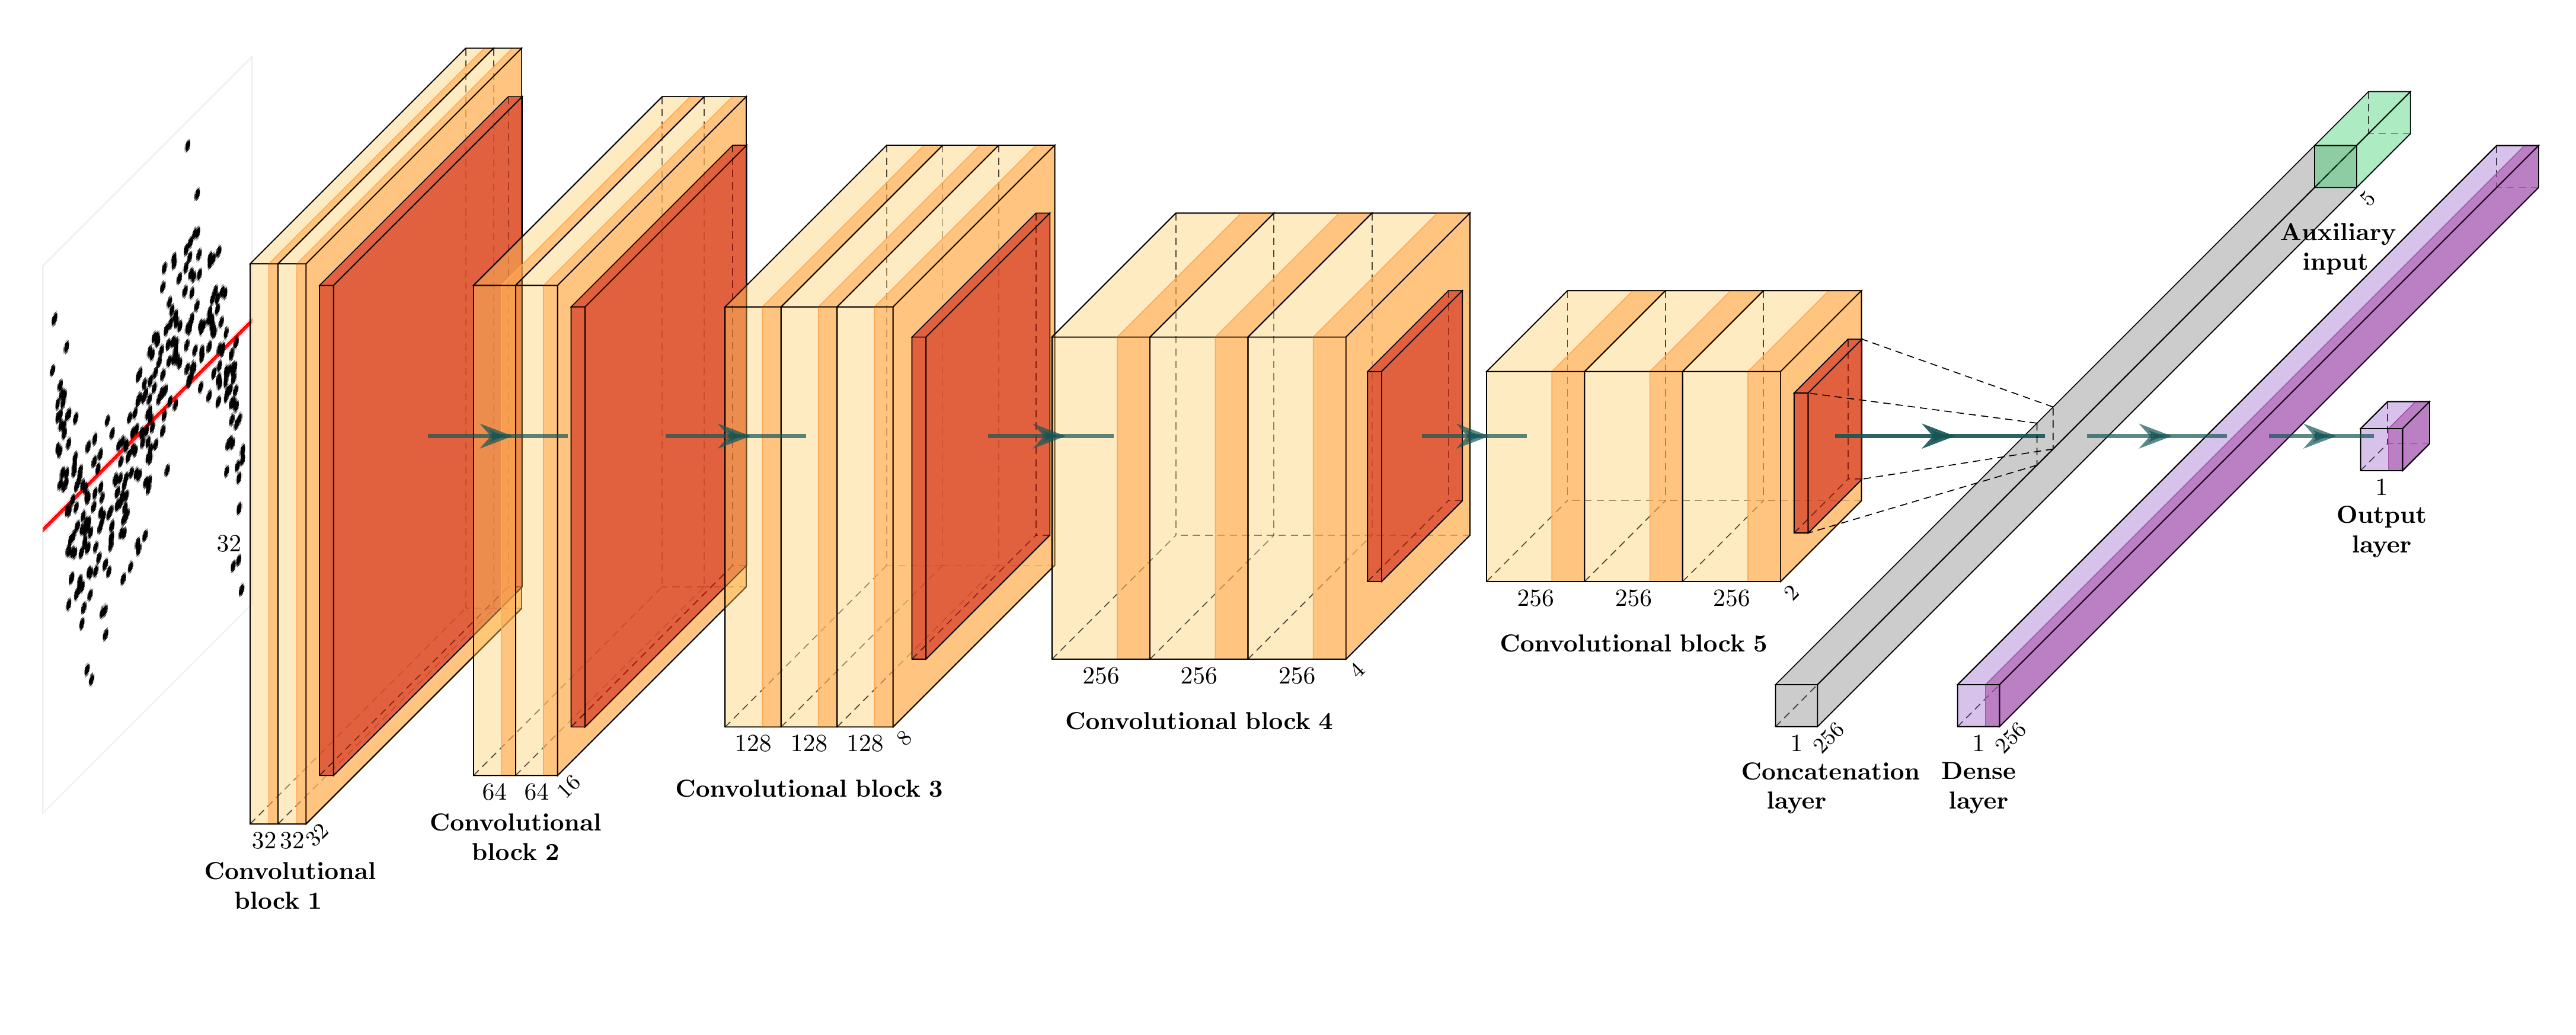
\includegraphics[width=1\linewidth]{paper_files/figure-latex/cnn-diag-1} 

}

\caption{Diagram of the architecture of the optimized computer vision model. Numbers at the bottom of each box show the shape of the output of each layer. The band of each box drawn in a darker color indicates the use of the rectified linear unit activation function.  Yellow boxes are 2D convolutional layers, orange boxes are pooling layers, the grey box is the concatenation layer, and the purple boxes are dense layers.}\label{fig:cnn-diag}
\end{figure}

The architecture of the computer vision model \(f_{CV}\) is adapted from
the well-established VGG16 architecture \citep{simonyan2014very}. While
more recent architectures like ResNet \citep{he2016deep} and
DenseNet\citep{huang2017densely}, have achieved even greater
performance, VGG16 remains a solid choice for many applications due to
its simplicity and effectiveness. Our decision to use VGG16 aligns with
our goal of starting with a proven and straightforward model. Figure
\ref{fig:cnn-diag} provides a diagram of the architecture. More details
about the neural network layers used in this study are provided in the
Appendix B.

The model begins with an input layer of shape
\(n \times h \times w \times 3\), capable of handling \(n\) RGB images.
This is followed by a grayscale conversion layer using the luma formula
under the Rec. 601 standard \citep{series2011studio}, which converts the
color image to grayscale. Grayscale suffices for our task since data
points are plotted in black. We experiment with three combinations of
\(h\) and \(w\): \(32 \times 32\), \(64 \times 64\), and
\(128 \times 128\), aiming to achieve sufficiently high image resolution
for the problem at hand.

The processed image is used as the input for the first convolutional
block. The model comprises at most five consecutive convolutional
blocks, mirroring the original VGG16 architecture. Within each block,
there are two 2D convolutional layers followed by two activation layers,
respectively. Subsequently, a 2D max-pooling layer follows the second
activation layer. The 2D convolutional layer convolves the input with a
fixed number of \(3 \times 3\) convolution filters, while the 2D
max-pooling layer downsamples the input along its spatial dimensions by
taking the maximum value over a \(2 \times 2\) window for each channel
of the input. The activation layer employs the rectified linear unit
(ReLU) activation function, a standard practice in deep learning, which
introduces a non-linear transformation of the output of the 2D
convolutional layer. Additionally, to regularize training, a batch
normalization layer is added after each 2D convolutional layer and
before the activation layer. Finally, a dropout layer is appended at the
end of each convolutional block to randomly set some inputs to zero
during training, further aiding in regularization.

The output of the last convolutional block is summarized by either a
global max-pooling layer or a global average-pooling layer, resulting in
a two-dimensional tensor. To enrich predictions with additional
information beyond visual features, this tensor is concatenated with an
additional \(n \times 5\) tensor, which contains the ``Monotonic'',
``Sparse'', ``Splines'', and ``Striped'' measures computed using the
\texttt{cassowaryr} R package \citep{mason2022cassowaryr} , along with
the number of observations for \(n\) residual plots. These measures were
selected for their reliability and efficiency, as other scagnostics
occasionally caused R process crashes (\(\sim 5\%\)) during data
preparation due to a bug in the \texttt{interp} package
\citep{Albrecht2023interp}. Although this bug was later fixed at our
request, the fix came too late to re-train the model. Moreover, their
high computational cost makes them unsuitable for fast inference.

The concatenated tensor is then fed into the final prediction block.
This block consists of two fully-connected layers. The first layer
contains at least \(128\) units, followed by a dropout layer. A batch
normalization layer is inserted between the fully-connected layer and
the dropout layer for regularization purposes. The second
fully-connected layer consists of only one unit, serving as the output
of the model.

The model weights \(\boldsymbol{\theta}\) were randomly initialized
using the Glorot Uniform method \citep{glorot2010understanding} and they
were optimized by the Adam optimizer \citep{kingma2014adam} with the
mean square error loss function

\[\hat{\boldsymbol{\theta}} = \underset{\boldsymbol{\theta}}{\text{arg min}}\frac{1}{n_{\text{train}}}\sum_{i=1}^{n_{\text{train}}}(D_i - f_{\boldsymbol{\theta}}(V_i, S_i))^2,\]

\noindent where \(n_{\text{train}}\) is the number of training samples,
\(V_i\) is the \(i\)-th residual plot and \(S_i\) is the auxiliary
information about the \(i\)-th residual plot including four scagnostics
and the number of observations.

\section{Data Generation and Model
Training}\label{sec-model-data-generation}

To enable supervised training of computer vision models for detecting
violations in linear regression, we generated a synthetic dataset of
80,000 training and 8,000 test residual plots. This simulation-based
approach provided full control over the data-generating process,
allowing precise computation of \(D\), cost-effective data scaling, and
the ability to model diverse visual patterns of model violations.

The simulated data incorporated three common types of residual
departures: non-linearity, heteroskedasticity, and non-normality. These
were introduced by fitting a standard simple linear regression model to
data generated from a more flexible model based on Hermite polynomials
\citep{hermite1864nouveau}, multiple predictors, and varying
distributions in both predictors and error terms. A comprehensive grid
of parameter combinations was explored to generate a wide range of
residual patterns. Importantly, the simulation included scenarios with
multiple violations occurring simultaneously. To ensure uniform coverage
across the difficulty scale of the target variable \(D\), a bucket
sampling scheme was used to create a balanced dataset. Samples were
iteratively simulated and accepted into one of 50 buckets, each
representing a distinct range of \(D\).

Model training was conducted on the MASSIVE M3 high-performance
computing platform \citep{goscinski2014multi} using TensorFlow
\citep{abadi2016tensorflow} and Keras \citep{chollet2015keras}.
Hyperparameters were optimized via Bayesian tuning with KerasTuner
\citep{omalley2019kerastuner}, minimizing validation RMSE across 100
trials. The tuning process included early stopping and considered
dropout rate, batch normalization, input resolution, and auxiliary
inputs.

Further details, including mathematical formulations of the synthetic
data model, parameter specifications, sampling scheme, example residual
plots and hyperparameter tuning configuration, are provided in the
Appendix A and C.

\section{Results}\label{sec-model-results}

\subsection{Model Performance}\label{model-performance}

Table \ref{tab:performance} summarizes the test performance of optimized
models using three input sizes. The \(32 \times 32\) model consistently
outperformed others, with a mean absolute error of approximately
\(0.43\), a negligible deviation given the typical \(D\) range of \(0\)
to \(7\). High \(R^2\) values also indicated strong linear correlation
between predictions and targets. Based on these results, we used the
best-performing \(32 \times 32\) model for subsequent analyses.

Figure \ref{fig:model-performance} shows a hexagonal heatmap of
\(D - \hat{D}\) versus \(D\). Smoothing curves (fitted by generalized
additive models \citep{hastie2017generalized}) reveal that all models
performed well for \(1.5 < D < 6\), where no structural issues were
observed. Over-prediction occurred when \(D < 1.5\), and
under-prediction primarily when \(\hat{D} > 6\).

For null plots (\(D = 0\)), over-prediction was expected (see Section
\ref{sec-model-lineup-evaluation}), but not under-prediction. Therefore,
we analysed the relationship between residuals and all the factors
involved in the data generating process. We found that most deviations
stemmed from non-linearity and the presence of a second predictor in the
synthetic data model, where small \(\varepsilon\) variances caused
under-predictions and large \(\varepsilon\) variances caused
over-prediction, as illustrated in Figure \ref{fig:over-under}.

To investigate further, we stratified the test set by violation type and
re-evaluated performance (Table \ref{tab:performance-sub}). It was found
that null plots had the poorest metrics, while non-normality cases were
easiest to predict, with RMSE around \(0.3\). Non-linearity
(\(\text{RMSE} \approx  0.8\)) was harder to assess than
heteroskedasticity (\(\text{RMSE} \approx  0.6\)) or non-normality
(\(\text{RMSE} \approx  0.3\)). Plots with multiple violations showed
intermediate performance.

\begin{table}

\caption{\label{tab:performance}The test performance of three optimized models with different input sizes.}
\centering
\begin{tabular}[t]{lrrrr}
\toprule
 & RMSE & $R^2$ & MAE & Huber loss\\
\midrule
$32 \times 32$ & 0.660 & 0.901 & 0.434 & 0.18\\
$64 \times 64$ & 0.674 & 0.897 & 0.438 & 0.19\\
$128 \times 128$ & 0.692 & 0.892 & 0.460 & 0.20\\
\bottomrule
\end{tabular}
\end{table}

\begin{figure}[!h]

{\centering 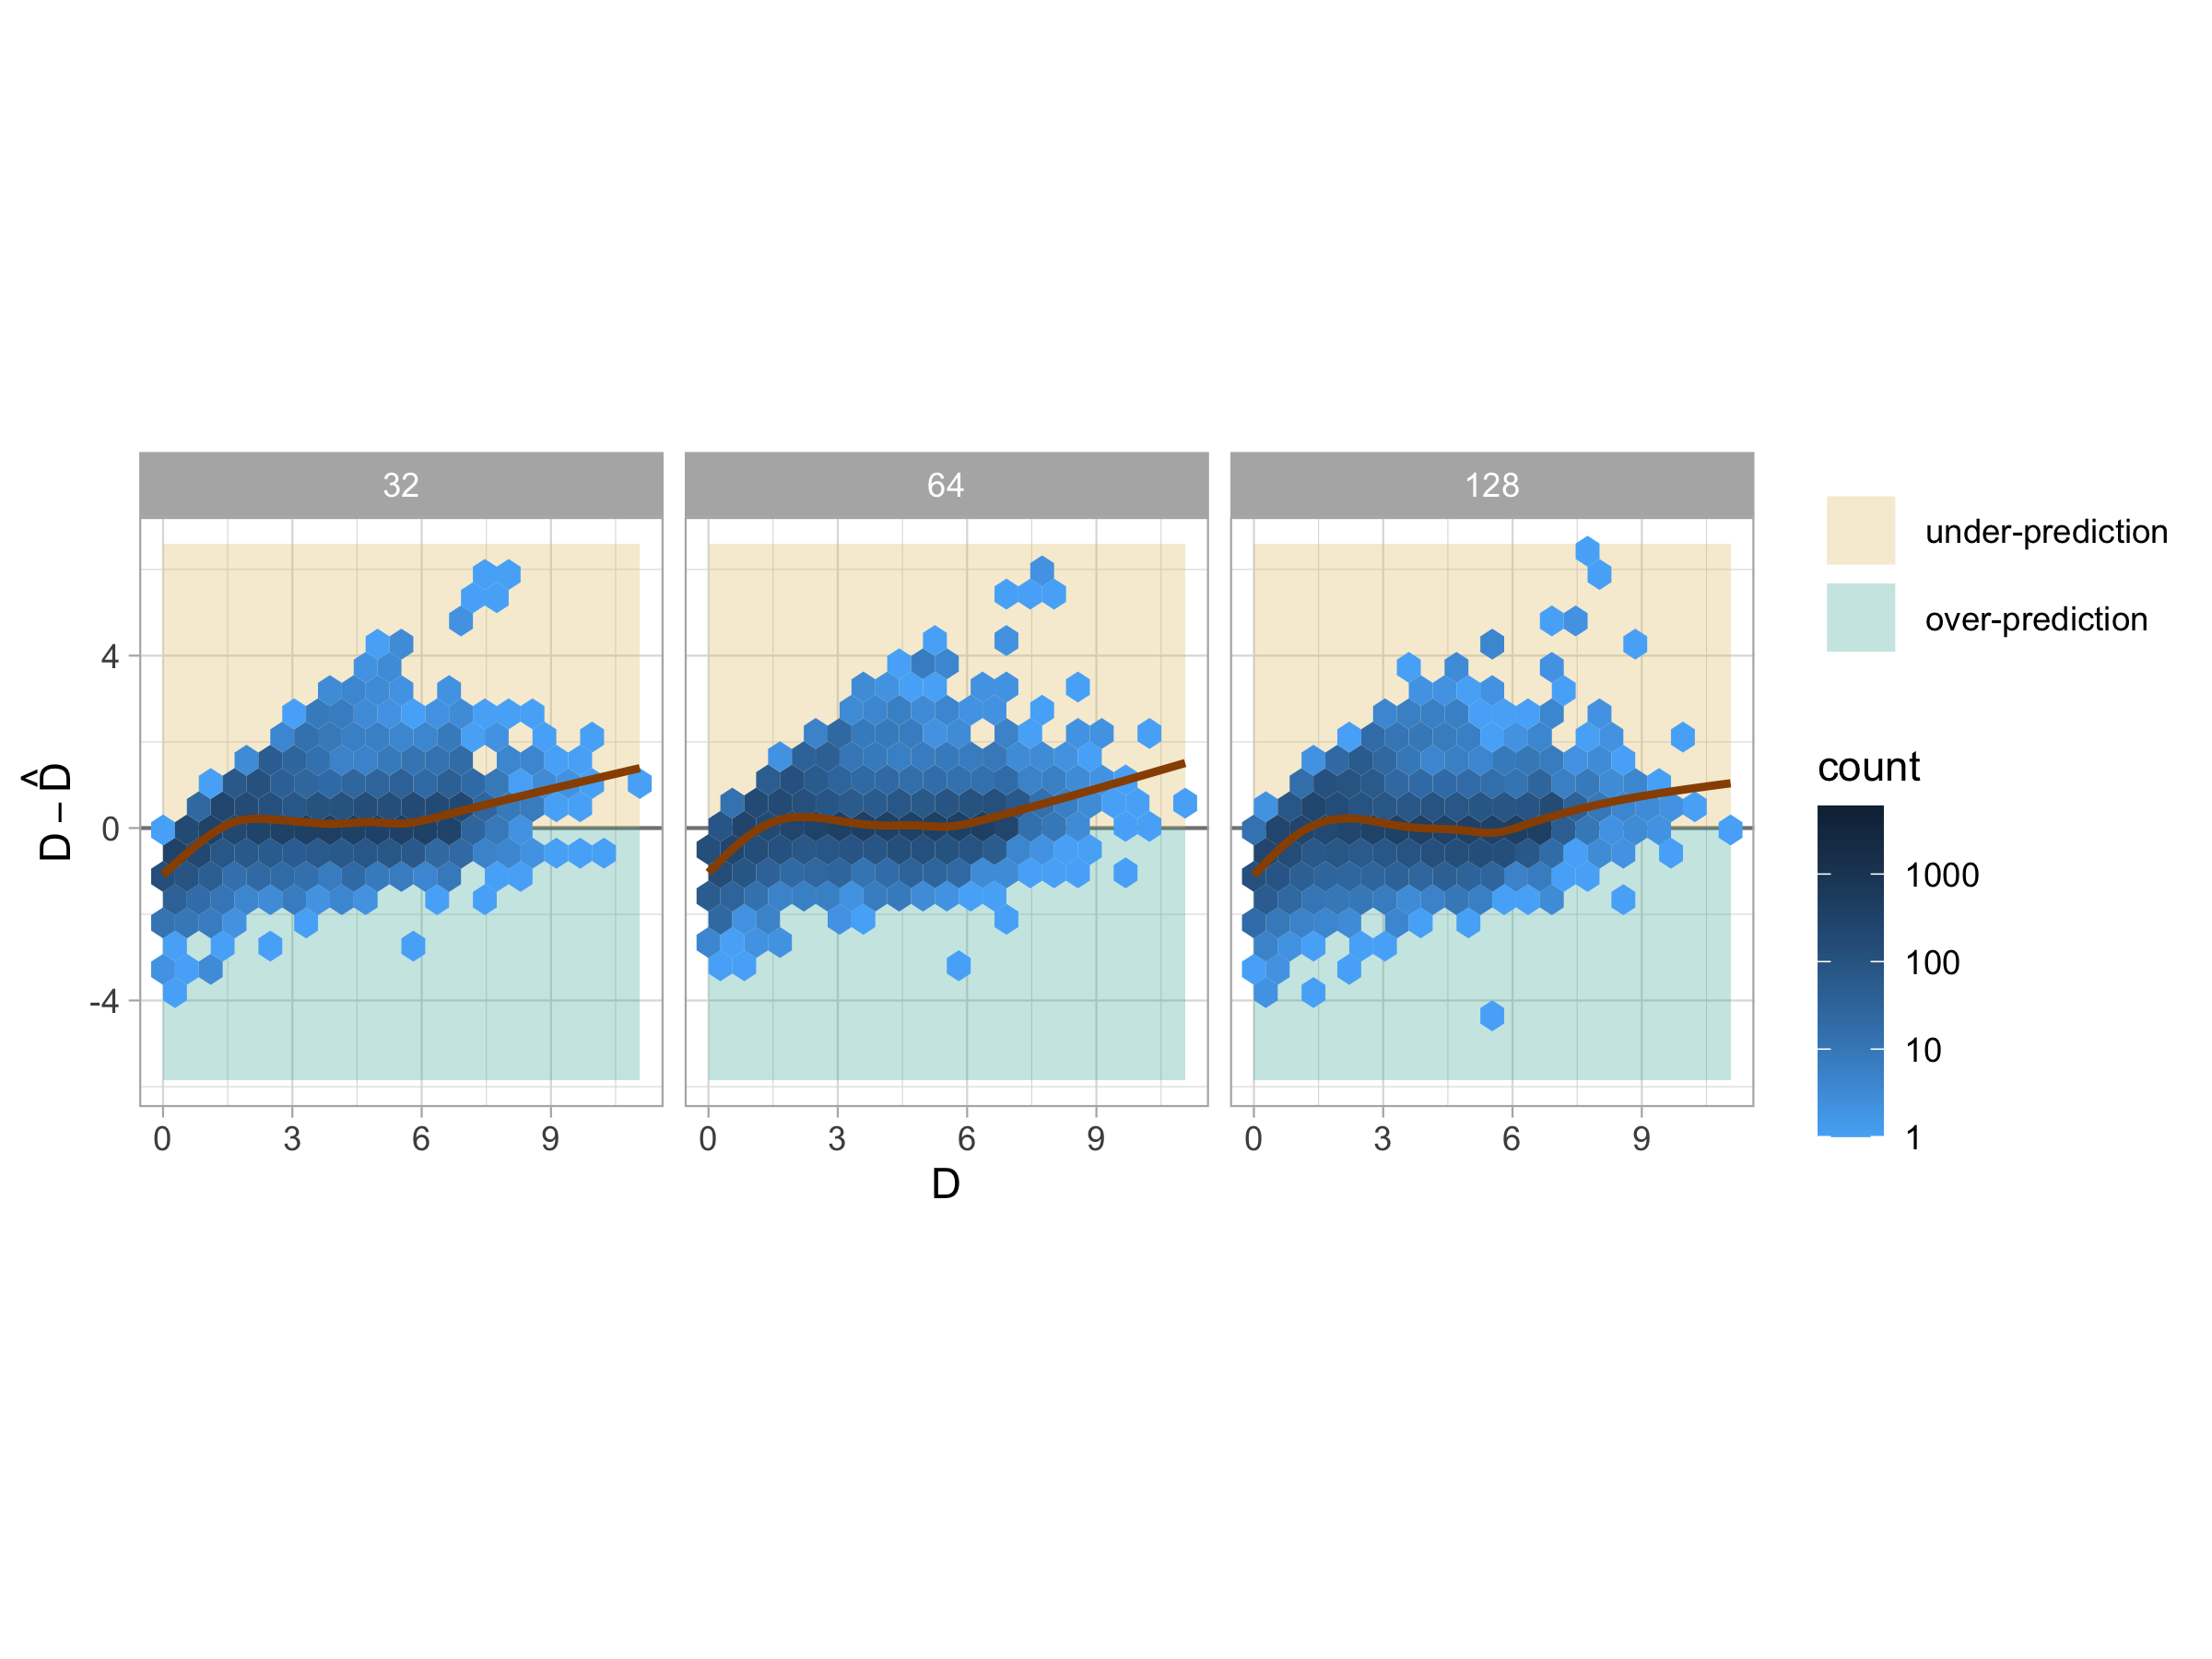
\includegraphics[width=1\linewidth]{paper_files/figure-latex/model-performance-1} 

}

\caption{Hexagonal heatmap for difference in $D$ and $\hat{D}$ vs $D$ on test data for three optimized models with different input sizes. The brown lines are smoothing curves produced by fitting generalized additive models. The area over the zero line in light yellow indicates under-prediction, and the area under the zero line in light green indicates over-prediction.}\label{fig:model-performance}
\end{figure}

\begin{figure}[!h]

{\centering 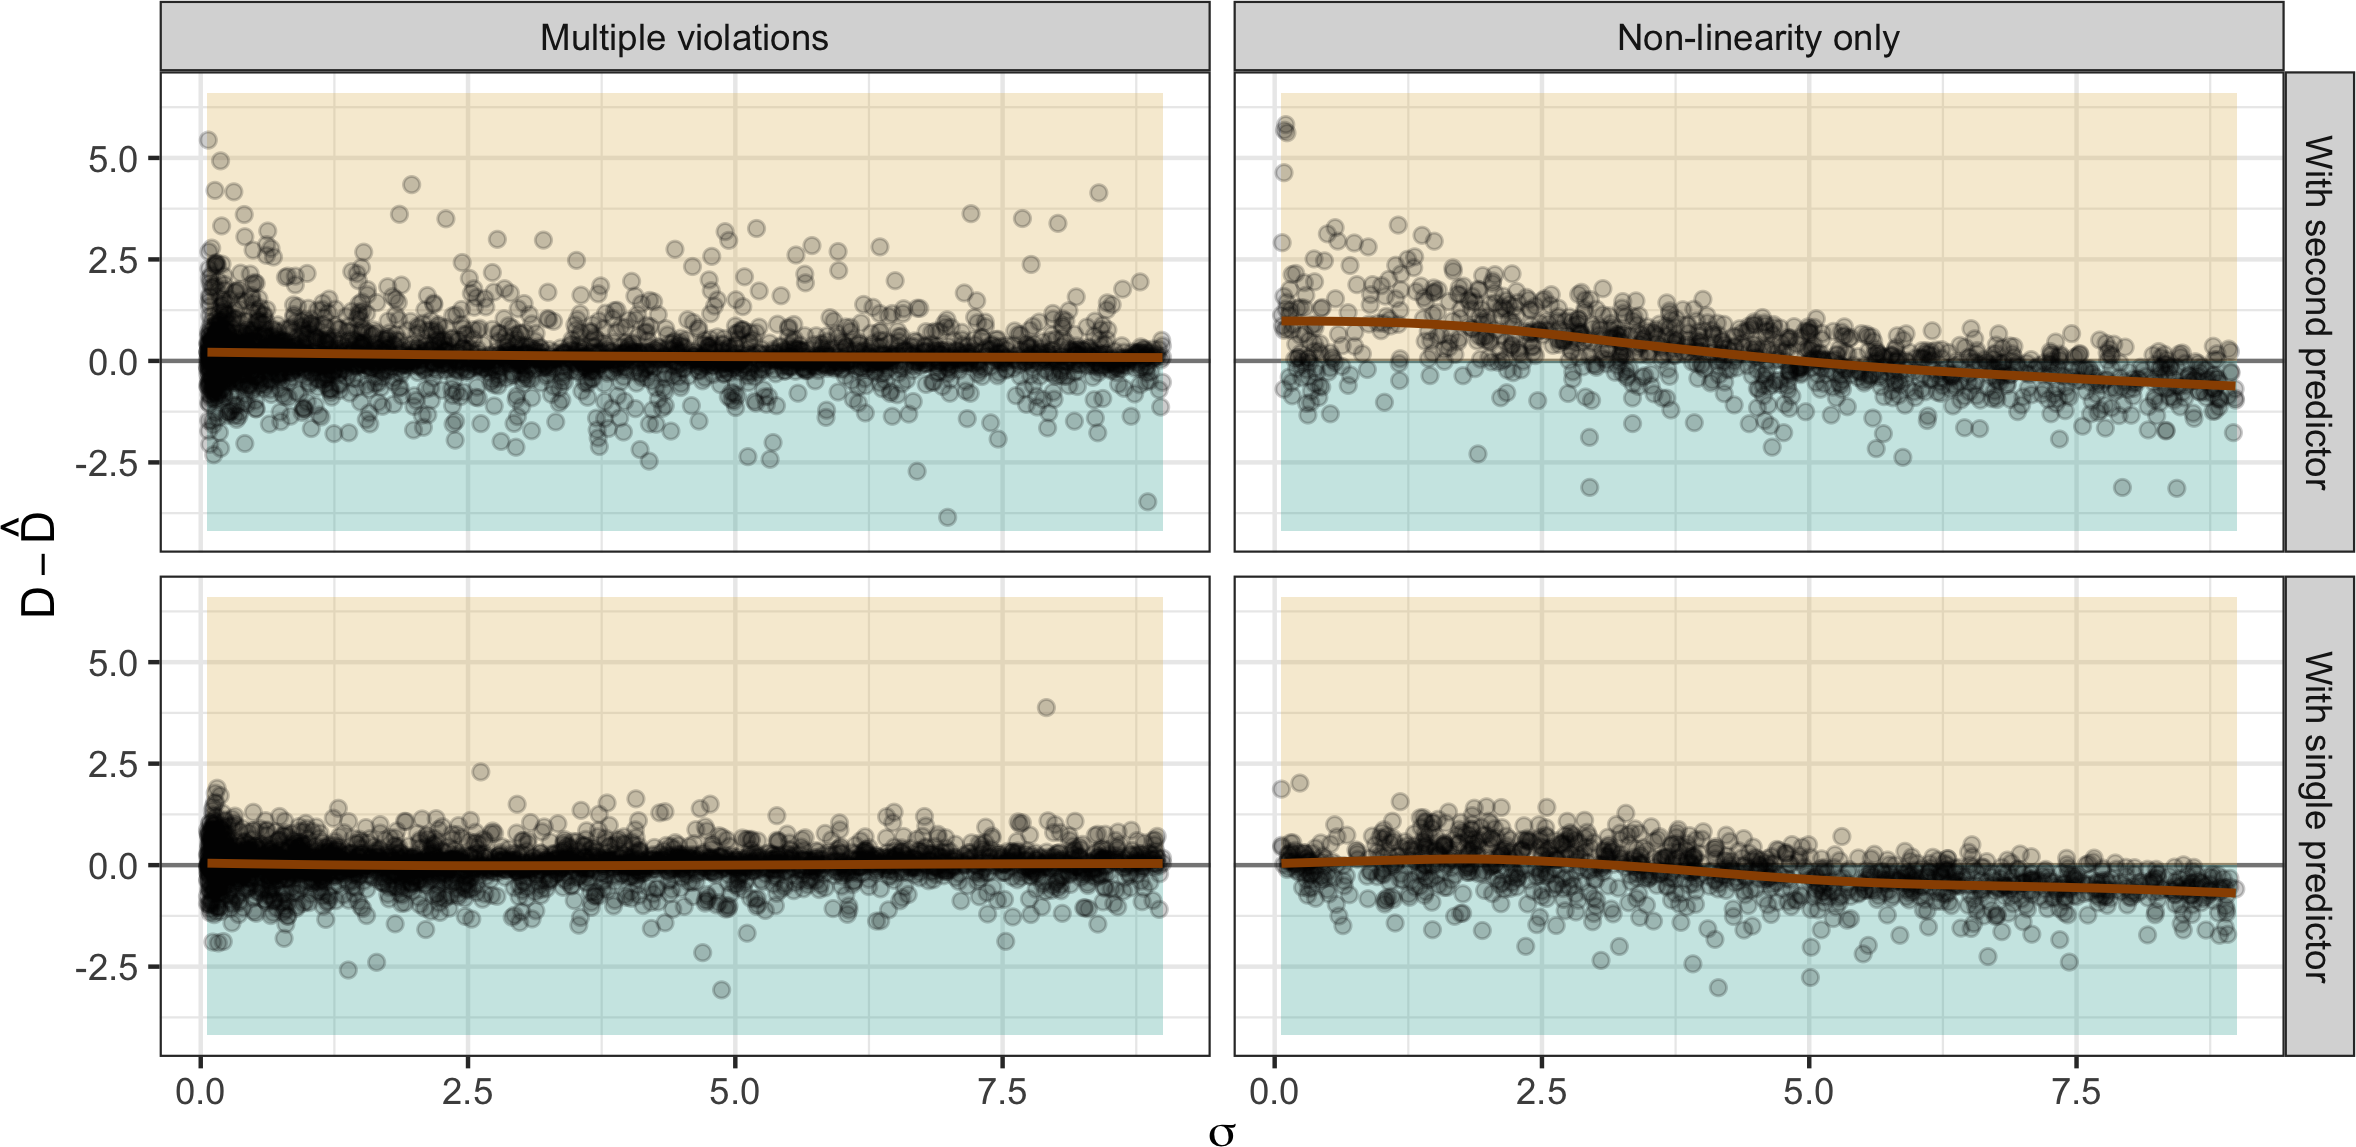
\includegraphics[width=1\linewidth]{paper_files/figure-latex/over-under-1} 

}

\caption{Scatter plots for difference in $D$ and $\hat{D}$ vs $\sigma$ on test data for the $32 \times 32$ optimized model. The data is grouped by whether the regression has only non-linearity violation, and whether it includes a second predictor in the regression formula. The brown lines are smoothing curves produced by fitting generalized additive models. The area over the zero line in light yellow indicates under-prediction, and the area under the zero line in light green indicates over-prediction.}\label{fig:over-under}
\end{figure}

\begin{table}

\caption{\label{tab:performance-sub}The test performance of the $32 \times 32$ model presented with different model violations.}
\centering
\begin{tabular}[t]{lrr}
\toprule
Violations & \#samples & RMSE\\
\midrule
no violations & 155 & 1.267\\
non-linearity & 2218 & 0.787\\
heteroskedasticity & 1067 & 0.602\\
non-linearity + heteroskedasticity & 985 & 0.751\\
non-normality & 1111 & 0.320\\
non-linearity + non-normality & 928 & 0.600\\
heteroskedasticity + non-normality & 819 & 0.489\\
non-linearity + heteroskedasticity + non-normality & 717 & 0.620\\
\bottomrule
\end{tabular}
\end{table}

\subsection{Comparison with Human Visual Inference and Conventional
Tests}\label{comparison-with-human-visual-inference-and-conventional-tests}

\subsubsection{Overview of the Human Subject
Experiment}\label{overview-of-the-human-subject-experiment}

In order to check the validity of the proposed computer vision model,
residual plots presented in the human subject experiment conducted by
\citet{li2024plot} will be assessed.

This study has collected 7,974 human responses to 1,152 lineups. Each
lineup contains one randomly placed true residual plot and 19 null
plots. Among the 1,152 lineups, 24 are attention check lineups in which
the visual patterns are designed to be extremely obvious and very
different from the corresponding to null plots, 36 are null lineups
where all the lineups consist of only null plots, 279 are lineups with
uniform predictor distribution evaluated by 11 participants, and the
remaining 813 are lineups with discrete, skewed or normal predictor
distribution evaluated by 5 participants. Attention check lineups and
null lineups will not be assessed in the following analysis.

In \citet{li2024plot}, the residual plots are simulated from a data
generating process that corresponds to a special case of the synthetic
data model used in this study. A key feature of the design is that model
violations are introduced independently, meaning non-linearity and
heteroskedasticity do not co-exist within a single lineup but are
instead assigned uniformly across different lineups. Moreover, the
experimental design does not account for non-normality or multiple
predictors.

\subsubsection{Model Performance on the Human-evaluated
Data}\label{model-performance-on-the-human-evaluated-data}

\begin{table}

\caption{\label{tab:experiment-performance}The performance of the $32 \times 32$ model on the data used in the human subject experiment.}
\centering
\begin{tabular}[t]{lrrrr}
\toprule
Violation & RMSE & $R^2$ & MAE & Huber loss\\
\midrule
heteroskedasticity & 0.721 & 0.852 & 0.553 & 0.235\\
non-linearity & 0.738 & 0.770 & 0.566 & 0.246\\
\bottomrule
\end{tabular}
\end{table}

Each lineup in \citet{li2024plot} contains one true residual plot and 19
null plots. While the true residual plot's distance \(D\) depends on the
data-generating process, null plots have \(D = 0\). We used our
optimized computer vision model to estimate \(D\) for all plots. To
ensure fair comparison, we reject \(H_0\) if the true residual plot has
the highest estimated distance. Conventional tests, including the Ramsey
RESET \citep{ramsey1969tests} for non-linearity and the Breusch-Pagan
test \citep{breusch1979simple} for heteroskedasticity, were also applied
to the same data.

Table \ref{tab:experiment-performance} reports performance metrics for
\(\hat{D}\) on true residual plots. While the performance is slightly
worse than on the test data provided in Table \ref{tab:performance}, the
mean absolute error remains low and the correlation between predictions
and true values remains high. Consistent with results in Table
\ref{tab:performance-sub}, non-linearity cases are harder to predict
than heteroskedasticity cases.

To assess how well the model's decisions align with other methods, Table
\ref{tab:human-conv-table} compares its rejection decisions with those
of conventional tests and human visual tests. Agreement rates are
85.95\% for heteroskedasticity cases and 79.69\% for non-linearity
cases, higher than those observed for human visual tests (67.96\% and
66.84\%, respectively). This suggests that the model aligns more closely
with the best available conventional tests. However, as Figure
\ref{fig:conv-mosaic} shows, the model does not always reject when
conventional tests do, indicating a lower sensitivity to model
violations.

To further illustrate these patterns, Figure \ref{fig:pcp} presents
parallel coordinate plots comparing decisions from human visual tests,
the computer vision model, and conventional tests. All three agree in
about 50\% of cases. When humans do not reject, conventional tests
reject in about half of those cases, whereas the model rejects in only
25\%. Notably, the model rarely rejects when both humans and
conventional tests do not, suggesting that while it is more sensitive
than humans, its rejection behavior is more aligned with human judgment
than with conventional tests.

Figure \ref{fig:power} plots rejection decisions against the true
distance \(D\). Compared to conventional tests, the computer vision
model rejects fewer cases when \(D < 4\), but a similar number of cases
when \(D > 4\). This indicates that the model is less sensitive to minor
deviations from model assumptions, while remaining comparably sensitive
to more substantial violations. Visual tests are the least sensitive
overall, showing few rejections for \(D < 2\), and requiring a higher
threshold (\(D > 5\)) for near-universal rejection, compared to
\(D > 4\) for both the model and conventional tests.

Finally, the power curves in Figure \ref{fig:power} are fitted using
logistic regression without intercepts and with an offset of
\(\log(0.05/0.95)\) to ensure a 5\% rejection rate under \(H_0\). The
model's rejection curve consistently lies between those of conventional
and human visual tests, indicating potential to further align its
decision boundary with human visual assessment.

\subsubsection{\texorpdfstring{Adjusted
\(\delta\)-difference}{Adjusted \textbackslash delta-difference}}\label{adjusted-delta-difference}

In the experiment conducted by \citet{li2024plot}, participants could
select multiple plots per lineup. To reflect detection confidence, a
weighted detection rate was computed for each lineup: selecting zero
plots yielded a weight of 0.05; otherwise, if the true residual plot was
selected, its weight was \(1 / \text{(number of selections)}\).

To evaluate the proposed distance measure, we could examine the
relationship between the weighted detection rate and the
\(\delta\)-difference statistic from \citet{chowdhury2018measuring}:

\[
\delta = \bar{d}_{\text{true}} - \underset{j}{\text{max}}\left(\bar{d}_{\text{null}}^{(j)}\right) \quad \text{for}~j = 1,...,m-1,
\]

\noindent where \(\bar{d}_{\text{true}}\) is the mean distance between
the true residual plot and all null plots, and
\(\bar{d}_{\text{null}}^{(j)}\) is the mean distance from null plot
\(j\) to other nulls. These averages help address asymmetries in
pairwise distances.

However, our method only compares each plot to a theoretically ``good''
residual plot, making the original formulation inapplicable. Moreover,
since \(D_{\text{null}} = 0\) by definition and \(D\) can not be derived
from an image, we instead focus on \(\hat{D}\), the model-estimated
distance. This leads to the adjusted \(\delta\)-difference:

\[
\delta_{\text{adj}} = \hat{D} - \underset{j}{\text{max}}\left(\hat{D}_{\text{null}}^{(j)}\right) \quad \text{for}~j = 1,...,m-1,
\]

\noindent where \(\hat{D}_{\text{null}}^{(j)}\) is the estimated
distance for the \(j\)-th null plot, and \(m\) is the number of plots in
a lineup.

Figure \ref{fig:delta} displays the scatter plot of the weighted
detection rate against \(\delta_{\text{adj}}\). It shows that weighted
detection generally increases with \(\delta_{\text{adj}}\), especially
when it is positive. This suggests that the differences in \(\hat{D}\)
capture some aspect of the visual separability between the true and null
plots as perceived by humans, with larger positive differences generally
indicating greater distinctiveness. However, the considerable
variability in detection rates for similar \(\delta_{\text{adj}}\)
values implies that \(\hat{D}\) does not fully account for all factors
influencing human perception, and the alignment remains imperfect. A
negative \(\delta_{\text{adj}}\) suggests some null plots may appear
more visually distinctive to humans than the true residual plot. In some
instances, the weighted detection rate is close to one despite a
negative \(\delta_{\text{adj}}\). This discrepancy implies that the
distance measure may not perfectly reflect actual human behavior.

\begin{table}

\caption{\label{tab:human-conv-table}Summary of the comparison of decisions made by computer vision model with decisions made by conventional tests and visual tests conducted by human.}
\centering
\begin{tabular}[t]{lrrr}
\toprule
Violations & \#Samples & \#Agreements & Agreement rate\\
\midrule
\addlinespace[0.3em]
\multicolumn{4}{l}{\textbf{Compared with conventional tests}}\\
\hspace{1em}heteroskedasticity & 540 & 464 & 0.8593\\
\hspace{1em}non-linearity & 576 & 459 & 0.7969\\
\addlinespace[0.3em]
\multicolumn{4}{l}{\textbf{Compared with visual tests conducted by human}}\\
\hspace{1em}heteroskedasticity & 540 & 367 & 0.6796\\
\hspace{1em}non-linearity & 576 & 385 & 0.6684\\
\bottomrule
\end{tabular}
\end{table}

\begin{figure}[!h]

{\centering 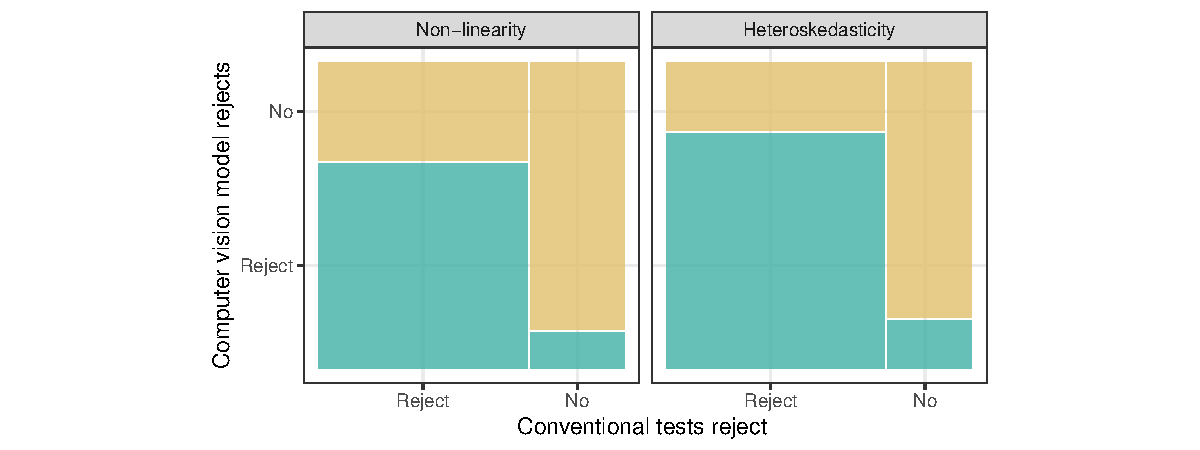
\includegraphics[width=1\linewidth]{paper_files/figure-latex/conv-mosaic-1} 

}

\caption{Rejection rate ($p$-value $\leq0.05$) of computer vision models conditional on conventional tests on non-linearity (left) and heteroskedasticity (right) lineups displayed using a mosaic plot. When the conventional test fails to reject, the computer vision mostly fails to reject the same plot as well as indicated by the height of the top right yellow rectangle, but there are non negliable amount of plots where the conventional test rejects but the computer vision model fails to reject as indicated by the width of the top left yellow rectangle.}\label{fig:conv-mosaic}
\end{figure}

\begin{figure}[!h]

{\centering 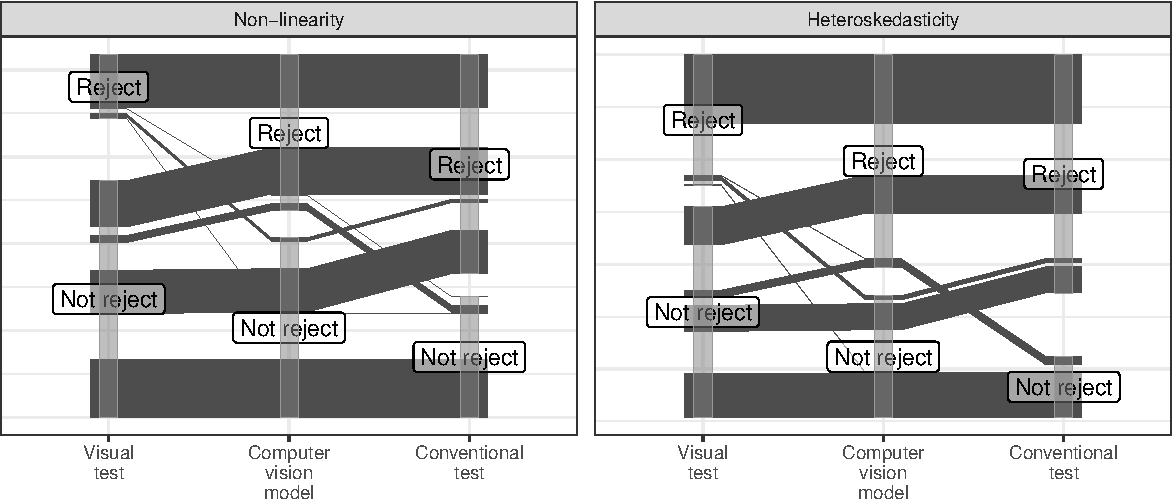
\includegraphics[width=1\linewidth]{paper_files/figure-latex/pcp-1} 

}

\caption{Parallel coordinate plots of decisions made by computer vision model, conventional tests and visual tests made by human.}\label{fig:pcp}
\end{figure}

\begin{figure}[!h]

{\centering 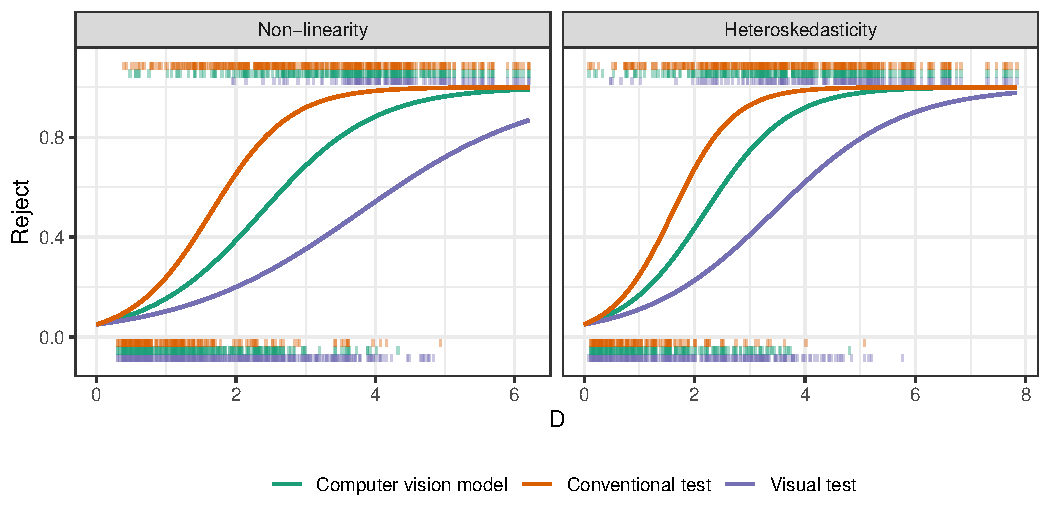
\includegraphics[width=1\linewidth]{paper_files/figure-latex/power-1} 

}

\caption{Comparison of power of visual tests, conventional tests and the computer vision model. Marks along the x-axis at the bottom of the plot represent rejections made by each type of test. Marks at the top of the plot represent acceptances. Power curves are fitted by logistic regression models with no intercept but an offset equals to $\text{log}(0.05/0.95)$.}\label{fig:power}
\end{figure}

\begin{figure}[!h]

{\centering 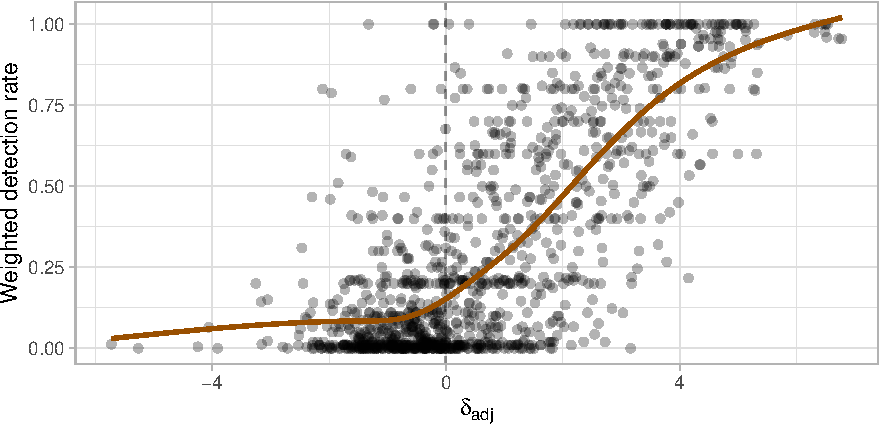
\includegraphics[width=0.8\linewidth]{paper_files/figure-latex/delta-1} 

}

\caption{A weighted detection rate vs adjusted $\delta$-difference plot. The brown line is smoothing curve produced by fitting generalized additive models.}\label{fig:delta}
\end{figure}

\section{Examples}\label{sec-examples}

In this section, we present the performance of the trained computer
vision model on three example datasets, including the dataset associated
with the residual plot displaying a ``left-triangle'' shape, the Boston
housing dataset \citep{harrison1978hedonic}, and the ``dino'' datasets
from the from the \texttt{datasauRus} package \citep{datasaurus}.

In the first case, both the model and human inspection correctly avoid
rejecting \(H_0\) when it is true, contrary to conventional tests,
highlighting the necessity of visual examination. The second case shows
a clear model violation detected by all tests, demonstrating the model's
practical use for less intricate tasks. The third case involves an
unusual deviation where the model and humans reject \(H_0\), but some
conventional tests do not, illustrating the benefits of visual-based
decision-making.

\subsection{Left-triangle}\label{left-triangle}

In Section \ref{sec-model-introduction}, we introduced a residual plot
(Figure \ref{fig:false-finding}) where the ``left-triangle'' shape could
be misinterpreted as evidence of heteroskedasticity. Although the
residuals are drawn from a correctly specified model, the Breusch-Pagan
test rejects \(H_0\) (\(p = 0.046\)). This visual artifact stems from
the skewed distribution of fitted values, as illustrated in the lineup
in Figure \ref{fig:lineup}A, where similar ``left-triangle'' patterns
appear across all residual plots. Since the true plot (at position 10)
is visually indistinguishable from the null plots, a visual test would
not reject \(H_0\).

The computer vision model yields a consistent conclusion. As shown in
Figure \ref{fig:false-check}, the estimated distance \(\hat{D}\) falls
well below the 95\% quantile of the null distribution, with a
\(p\)-value of \(0.33\). The bootstrapped distribution further suggests
that rejection of the fitted model is highly unlikely. Together, the
visual and model-based tests do not reject \(H_0\), in contrast to the
Breusch-Pagan test, which lacks the context provided by null plots and
may be misled by visual artifacts.

To further interpret the model's output, the attention map in Figure
\ref{fig:false-check}B, computed as the gradient of the output with
respect to the greyscale input, shows that the top-right and
bottom-right corners of the residual plot have the most influence,
corresponding to the triangle's vertices. In addition, a principal
component analysis (PCA) of the 256 features extracted by the model's
global pooling layer (Figure \ref{fig:false-check}D) shows that null and
bootstrapped plots cluster together in the space defined by the first
two principal components, and the true residual plot is covered by the
cluster. This overlap reinforces the conclusion that the true plot is
visually indistinct, aligning with our interpretation of the lineup.

\begin{figure}[!h]

{\centering 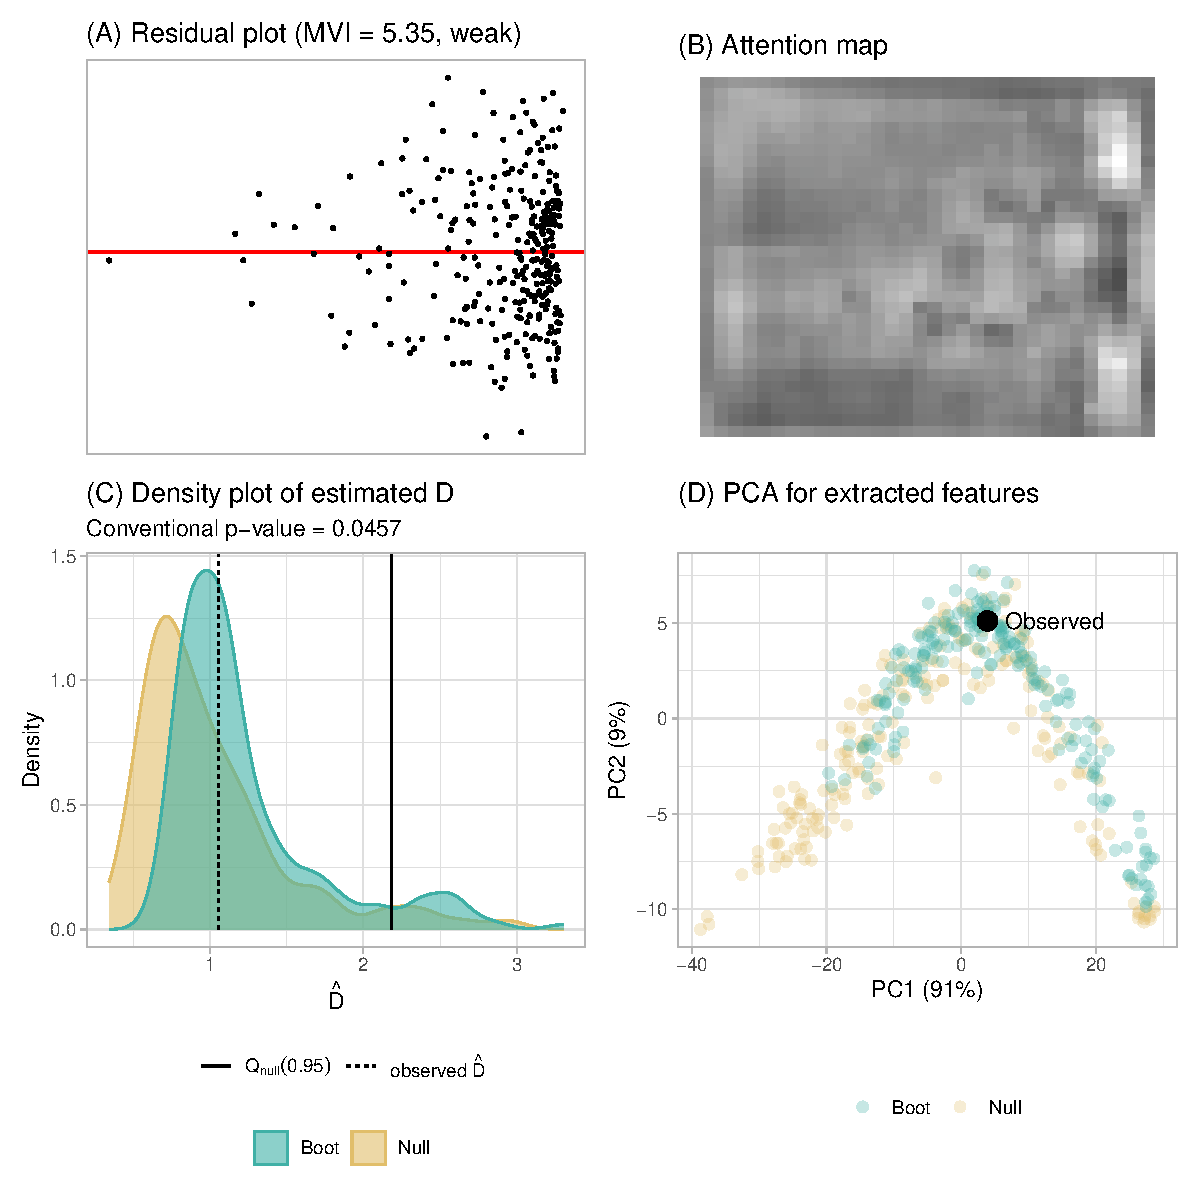
\includegraphics[width=0.8\linewidth]{paper_files/figure-latex/false-check-1} 

}

\caption{A summary of the residual plot assessment evaluted on 200 null plots and 200 bootstrapped plots. (A) The true residual plot exhibiting a "left-triangle" shape. (B) The attention map produced by computing the gradient of the output with respect to the greyscale input.  (C) The density plot of estimated distance for null plots and bootstrapped plots. The green area indicates the distribution of estimated distances for bootstrapped plots, while the yellow area represents the distribution of estimated distances for null plots. The fitted model will not be rejected since $\hat{D} < Q_{null}(0.95)$. (D) The scatter plot of first two principal components of features extracted from the global pooling layer of the computer vision model.  }\label{fig:false-check}
\end{figure}

\subsection{Boston Housing}\label{boston-housing}

The Boston housing dataset, originally published by
\citet{harrison1978hedonic}, provides insights into housing in the
Boston, Massachusetts area. For illustration, we use a reduced Kaggle
version containing 489 observations and four variables: average number
of rooms per dwelling (RM), percentage of lower status population
(LSTAT), pupil-teacher ratio by town (PTRATIO), and median home value
(MEDV). We fit a linear regression model with MEDV as the response and
the remaining variables as predictors, focusing on detecting
non-linearity, because the relationships between RM and MEDV or LSTAT
and MEDV are non-linear.

Figure \ref{fig:boston-check} summarizes the model evaluation. The
residual plot (Figure \ref{fig:boston-check}A) reveals a distinct
``U''-shaped pattern, suggesting non-linearity. The RESET test strongly
rejects \(H_0\) with a very small \(p\)-value, and the computer vision
model yields a large estimated distance \(\hat{D}\), well above the 95\%
quantile of the null distribution (\(p\text{-value} = 0.00498\)). The
bootstrapped distribution also shows widespread rejection, indicating
the model is likely misspecified. The attention map (Figure
\ref{fig:boston-check}B) highlights the central region of the residual
plot, corresponding to the turning point of the ``U'', as most
influential. In the PCA projection (Figure \ref{fig:boston-check}D),
bootstrapped and null plots form two distinct clusters, emphasizing the
visual separability. This aligns with the lineup in Figure
\ref{fig:lineup}B, where the true plot stands out clearly. A human
visual test would also likely reject \(H_0\) in this case.

\begin{figure}[!h]

{\centering 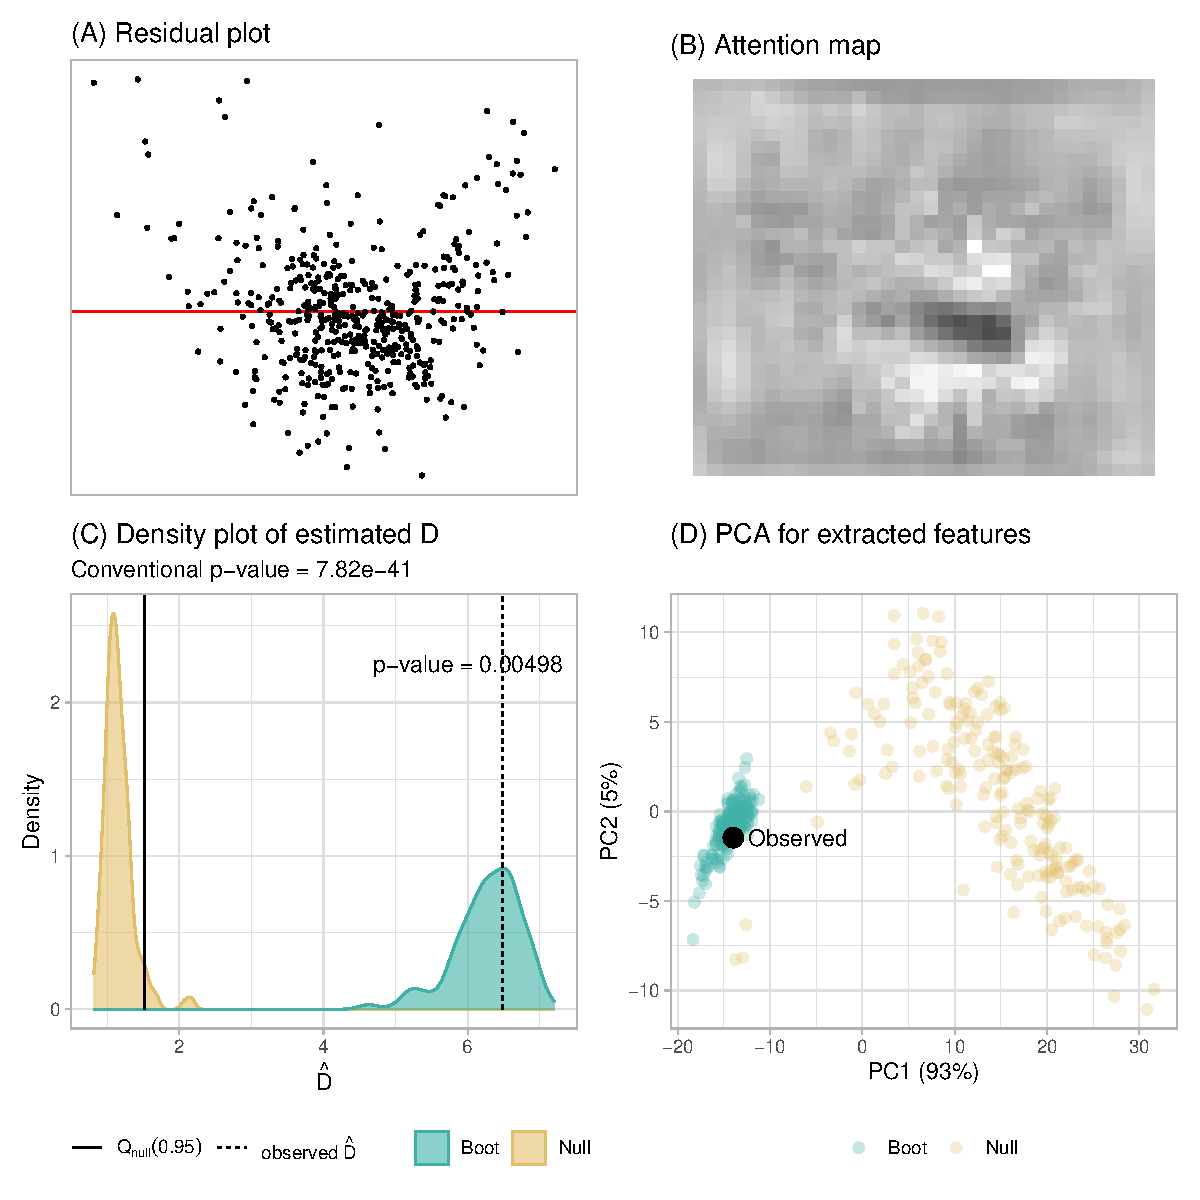
\includegraphics[width=0.8\linewidth]{paper_files/figure-latex/boston-check-1} 

}

\caption{A summary of the residual plot assessment for the Boston housing fitted model evaluted on 200 null plots and 200 bootstrapped plots. (A) The true residual plot exhibiting a "U" shape. (B) The attention map produced by computing the gradient of the output with respect to the greyscale input.  (C) The density plot of estimated distance for null plots and bootstrapped plots. The blue area indicates the distribution of estimated distances for bootstrapped plots, while the yellow area represents the distribution of estimated distances for null plots. The fitted model will be rejected since $\hat{D} \geq Q_{null}(0.95)$. (D) The scatter plot of first two principal components of features extracted from the global pooling layer of the computer vision model. }\label{fig:boston-check}
\end{figure}

\subsection{DatasauRus}\label{datasaurus}

Beyond detecting common issues like non-linearity, heteroskedasticity,
and non-normality, the computer vision model can also identify unusual
visual artifacts, such as shapes resembling real-world objects, as long
as such patterns do not appear in null plots. These cases are
challenging to categorize using conventional model diagnostics, so we
compare the model's output with results from the RESET test,
Breusch-Pagan test, and Shapiro-Wilk test \citep{shapiro1965analysis}.

The ``dino'' dataset from the \texttt{datasauRus} R package illustrates
this situation. It contains only two variables, \(x\) and \(y\), but
fitting a regression model produces a residual plot that clearly
resembles a dinosaur (Figure \ref{fig:dino-check}A). This pattern is
visually distinctive in the lineup shown in Figure \ref{fig:lineup}C,
where a human visual test would undoubtedly reject \(H_0\).

Consistent with this, the computer vision model assigns a distance
\(\hat{D}\) above the 95\% quantile of the null distribution
(\(p-\text{value} = 0.00498\)), leading to rejection of \(H_0\). The
bootstrapped distribution further supports this, with most fitted models
also being rejected. In contrast, the RESET and Breusch-Pagan tests
yield \(p\)-values above \(0.3\), suggesting no violation. Only the
Shapiro-Wilk test rejects normality with a small \(p\)-value.

Crucially, the attention map in Figure \ref{fig:dino-check}B highlights
the dinosaur shape, indicating that the model's decision is driven by
human-perceptible features. The model appears to capture contours and
outlines in a manner similar to human visual interpretation. In the PCA
plot (Figure \ref{fig:dino-check}D), the cluster of bootstrapped plots
is positioned at the corner of the cluster of null plots, isolated from
the cluster of null plots.

In practice, such visual artifacts would be difficult to detect without
inspecting the residual plot directly. Furthermore, analysts do not
always test for normality, and even when violations are found, they are
often deemed acceptable due to the robustness of linear regression under
quasi-likelihood theory. This example highlights the value of visual
diagnostics and the unique role of the proposed computer vision model in
supporting them.

\begin{figure}[!h]

{\centering 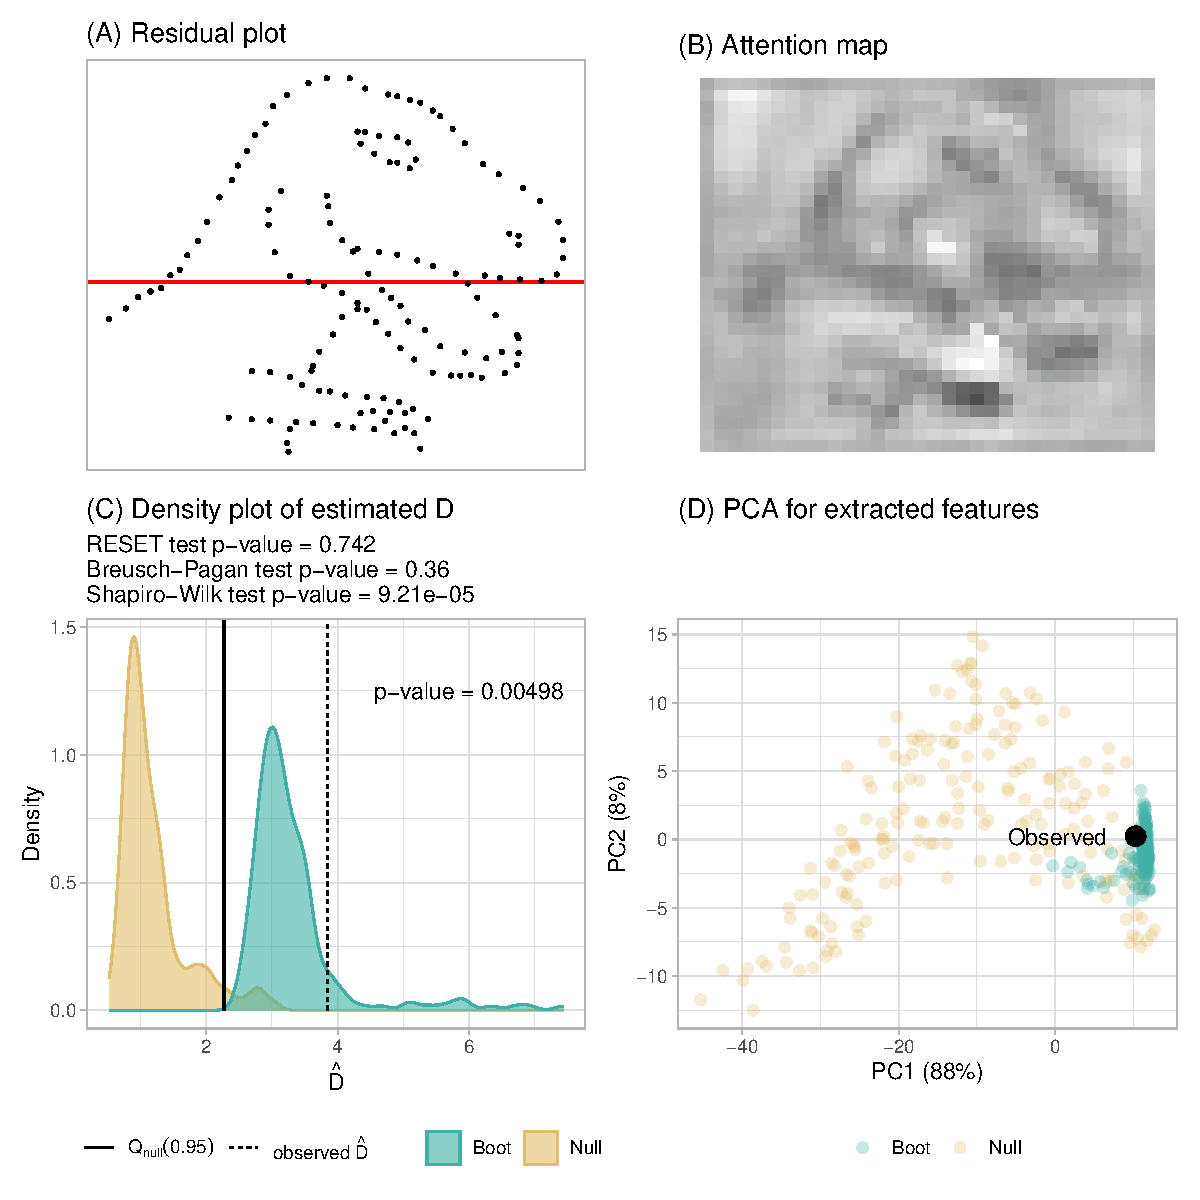
\includegraphics[width=0.8\linewidth]{paper_files/figure-latex/dino-check-1} 

}

\caption{A summary of the residual plot assessment for the datasauRus fitted model evaluated on 200 null plots and 200 bootstrapped plots. (A) The residual plot exhibits a "dinosaur" shape. (B) The attention map produced by computing the gradient of the output with respect to the greyscale input.  (C) The density plot of estimated distance for null plots and bootstrapped plots. The blue area indicates the distribution of estimated distances for bootstrapped plots, while the yellow area represents the distribution of estimated distances for null plots. The fitted model will be rejected since $\hat{D} \geq Q_{null}(0.95)$. (D) The scatter plot of first two principal components of features extracted from the global pooling layer of the computer vision model.}\label{fig:dino-check}
\end{figure}

\begin{figure}[!h]

{\centering 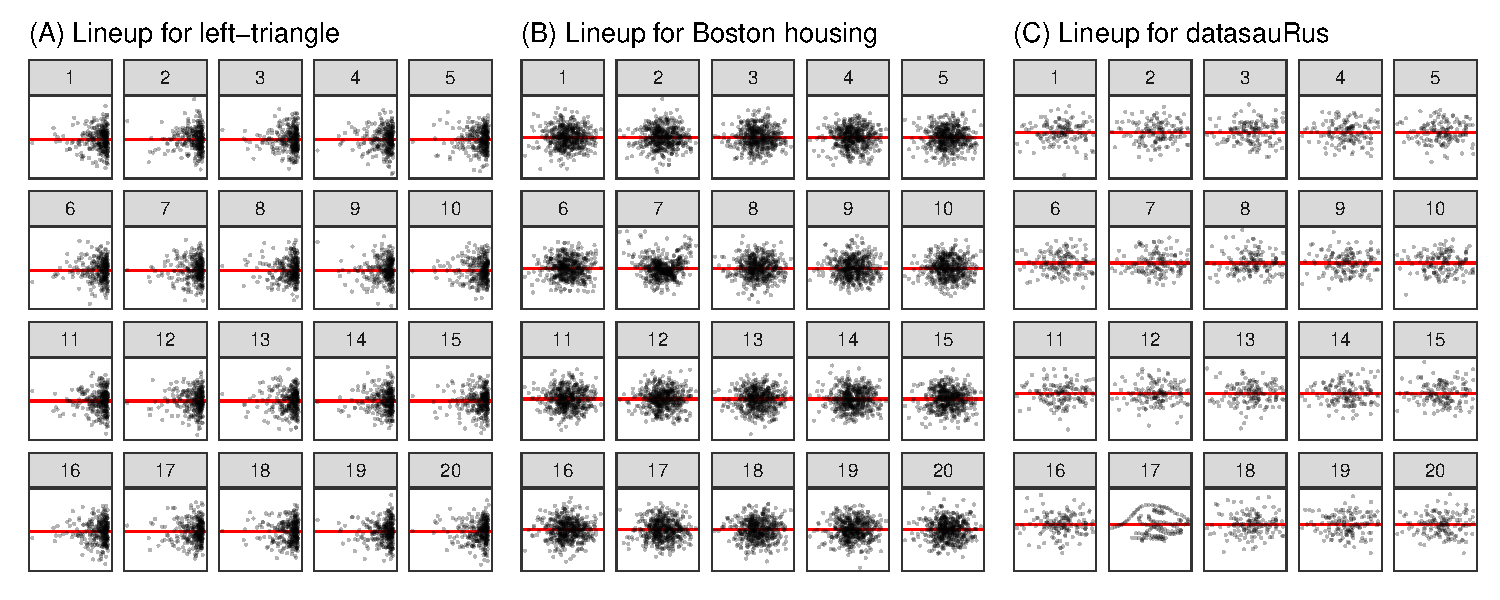
\includegraphics[width=1\linewidth]{paper_files/figure-latex/lineup-1} 

}

\caption{Lineups of residual plots for the "left-triangle", "Boston housing", and "datasauRus" datasets. (A) True plot at position 10; no clear visual difference. (B) True plot at position 7; clearly stands out. (C) True plot at position 17; distinctly artificial and easily identifiable.}\label{fig:lineup}
\end{figure}

\section{Limitations and Future Work}\label{limitations-and-future-work}

While the computer vision model performs well under the synthetic data
generation scheme and across the three illustrative examples, this study
has several limitations that point to directions for future work.

First, the proposed distance measure assumes the true model follows a
classical normal linear regression framework, which may be restrictive.
Although we do not explore relaxation of this assumption here, future
work could extend the approach to other types of regression models. One
possibility is to define a distance measure tailored to each model class
and re-train the computer vision model accordingly. To reduce
computational cost, the convolutional blocks from our current model
could be reused via transfer learning, as it is already effective at
capturing visual features. Alternatively, transforming residuals to
approximate normality and constant variance could allow for meaningful
comparisons under our current distance measure. However, if raw
residuals are used, the interpretation remains valid only when the
visual differences between the true and null plots are detectable by the
proposed distance measure.

Second, this study focused solely on the standard residuals vs.~fitted
values plot, leaving out other common diagnostic plots such as residuals
vs.~predictors and Q-Q plots. These alternative plots may offer
additional information and could be incorporated into a broader visual
testing framework in future research.

Finally, we chose a relatively simple computer vision architecture to
establish a baseline for automated visual inference. While the current
model shows promise, there is room to improve its alignment with human
judgment. Achieving this may require external data from surveys or
controlled experiments to better understand how human observers
interpret residual plots and how these judgments differ from the model's
outputs.

\section{Conclusions}\label{conclusions}

In this paper, we have introduced a distance measure based on the
Kullback-Leibler divergence to quantify disparity between the residual
distribution of a fitted classical normal linear regression model and
the reference distribution under correct specification. This measure
captures the extent of model violations and forms the basis of a
computer vision model that estimates the distance using residual plots
as input.

The estimated distance supports a formal statistical testing procedure
by comparing the true residual plot against null plots generated from
the fitted model. Through bootstrapping and model refitting, we also
evaluate how often a correctly specified model would be flagged as
misspecified under repeated sampling.

The trained computer vision model performs well on both training and
test data, though its performance is somewhat lower for non-linear
patterns. Statistical tests based on the model's predicted distance show
lower sensitivity than conventional tests but higher sensitivity than
human visual tests. Importantly, the predicted distance broadly aligns
with the strength of visual signals perceived by humans, though further
improvements are possible.

We demonstrate the method across several scenarios, highlighting its
effectiveness and its conceptual alignment with visual inference. Both
visual and distance-based tests act as omnibus procedures, detecting a
wide range of model violations collectively. In contrast, conventional
tests such as RESET and Breusch-Pagan target specific assumptions,
making them less flexible and potentially harder to combine without
adjusting for multiple testing.

Overall, our approach offers a practical tool to support regression
diagnostics by reducing the manual effort required for residual plot
inspection. While we recommend analysts to continue reading residual
plots whenever feasible, our method can augment the process, either as
an automated screening tool or a supplement to human judgment.

\section*{Supplementary Materials}\label{supplementary-materials}
\addcontentsline{toc}{section}{Supplementary Materials}

\begin{description}
\item{Appendix:} The appendix includes more details about the synthetic data generation process, neural network layers used in the work, model training, and model violation index. (appendix.pdf, Portable Document Format file)
\end{description}

\section*{Acknowledgement}\label{acknowledgement}
\addcontentsline{toc}{section}{Acknowledgement}

These \texttt{R} packages were used for the work: \texttt{tidyverse}
\citep{tidyverse}, \texttt{lmtest} \citep{lmtest}, \texttt{mpoly}
\citep{mpoly}, \texttt{ggmosaic} \citep{ggmosaic}, \texttt{kableExtra}
\citep{kableextra}, \texttt{patchwork} \citep{patchwork},
\texttt{rcartocolor} \citep{rcartocolor}, \texttt{glue} \citep{glue},
\texttt{ggpcp} \citep{ggpcp}, \texttt{here} \citep{here},
\texttt{magick} \citep{magick}, \texttt{yardstick} \citep{yardstick} and
\texttt{reticulate} \citep{reticulate}.

The article was created with R packages \texttt{rticles}
\citep{rticles}, \texttt{knitr} \citep{knitr} and \texttt{rmarkdown}
\citep{rmarkdown}. The project's GitHub repository
(\url{https://github.com/TengMCing/auto_residual_reading_paper})
contains all materials required to reproduce this article.

\section*{Disclosure Statement}\label{disclosure-statement}
\addcontentsline{toc}{section}{Disclosure Statement}

No potential conflict of interest was reported by the author(s).

\bibliographystyle{tfcad}
\bibliography{bibliography.bib}





\end{document}
